\documentclass[a4paper,11pt]{book}
\usepackage{makeidx}
\usepackage{graphicx}
\usepackage{amsfonts}
\usepackage{amssymb}
\usepackage{amsmath}
\usepackage{euscript}
\usepackage{boxedminipage}
\usepackage{lscape}
\usepackage{minitoc}
\usepackage{epsfig,psfrag,verbatim}
\usepackage{url,natbib}
\usepackage{booktabs, longtable}

\vfuzz2pt % Don't report over-full v-boxes if over-edge is small
\hfuzz2pt % Don't report over-full h-boxes if over-edge is small

\setlength{\oddsidemargin}{0cm}
\setlength{\evensidemargin}{0cm}
\setlength{\textwidth}{16cm}
\setlength{\textheight}{23cm}

\begin{document}
\title{Work package 8}
\author{}
\date{\today}
\maketitle
\tableofcontents

\subsubsection*{Acknowledgement}
This work was carried out in conjunction with the EURACE project (EU IST FP6
STREP grant 035086) which is a consortium lead by S. Cincotti (Universit\`{a} di
Genova), H. Dawid (Universitaet Bielefeld), C. Deissenberg (Universit\'{e} de la
M\'{e}diterran\'{e}e), K. Erkan (TUBITAK National Research Institute of Electronics
and Cryptology), M. Gallegati  (Universit\`{a} Politecnica delle Marche), M.
Holcombe (University of Sheffield), M. Marchesi (Universit\`{a} di Cagliari), C.
Greenough (STFC - Rutherford Appleton Laboratory).


\chapter{System of National Accounts}
%\chapter{System of National Accounts}

\section{Stock-flow consistent models}
An important part of the testing and verification process will be the verification of the internal consistency of the model. For this task we need a stock-flow consistent (SFC) model, that can be defined as:
\begin{quote}
``[...] models that identify economic agents with the main social categories/institutional sectors of actual capitalist economies -- thoroughly describe these agents' short-period behaviors and consistently model the `period by period' balance sheet dynamics implied by the latter.'' (\citet[p. 2]{Macedo-e-Silva:2008})
\end{quote}
Using a SFC model we need to check that all monetary flows are accounted for, and that all changes to stock variables are consistent with these flows. This can be accomplished by tracking the time evolution of the balance sheets across the different sectors of the economy. This could be done by constructing a Social Accounting Matrix (SAM) that contains all the monetary flows and changes to the balance sheet between the beginning and end of an accounting period. A SAM consists of a double-entry accounting system in which each flow comes from somewhere and goes to somewhere. It shows how the balance sheets of the different economic sectors (agents) are interlinked, and it also shows how the period-by-period balance sheets change dynamically over time. Such an accounting system at the macro level provides us with a number of accounting identities that should always hold and this can be tested by an external invariant detector such as Daikon.

This provides us with a solid and economically well-founded methodology to test the consistency of the model and it increases the credibility that can be attached to the model's results. Thereby it is not only part of the testing and verification procedure, but is also part of the accreditation process. It will help to raise the acceptability and trust in the model.

\section{Balance sheets}
Below we list for each agent type the items on its balance sheet. The cash flows indicated only relate to the financing activities.

\subsection{Household}
Table \ref{Table: Household balance sheet} and \ref{Table: Household cash flow}.

Households can have bank deposits ($M^h$) but they do not receive any interest ($r^{m} M^h=0$).
They can purchase government bonds ($B^h$) and private equity shares ($E^h$). They do not take out bank loans. They receive interest on the government bonds ($+r^gB^h$) and dividends on the shares ($+Div^h$). The equity transactions are denoted in this text as a share purchase by the household ($-SP^h$) or a share repurchase by the firm ($+SR^h$).

\subsection{Firm - CGP and IGP}
Table \ref{Table: Firm income statement},\ref{Table: Firm balance sheet},\ref{Table: Firm cash flow}.

Firms can have bank deposits ($M^f$) and bank loans ($L^f$). They do not receive any interest on the deposits ($r^{m} M^f=0$), but do have to pay interest on the loans ($r^b L^f$). They can also issue equity shares ($E^f$) on which they pay dividends ($-Div^f$). They can also do a share repurchase ($SR^f$). They they do not purchase government bonds, or shares of other firms.

\subsection{Bank}
%\subsection{Bank balance sheet}
Table \ref{Table: Bank balance sheet} and \ref{Table: Bank cash flow}.

Banks can issue equity shares on which they pay dividends ($E^b$, $-Div^b$). They have a portfolio of outstanding loans ($L^b$) on which they receive interest ($+r^b L^b$) and debt instalment payments ($-\Delta L^b$).
They do not purchase government bonds, and they do not purchase shares in other firms or banks. The banks have a standing facility with the Central Bank from which they can draw advances freely ($A^b$), on which they have to pay an interest to the Central Bank ($-r^{cb}A^b$).

\subsection{Government}
%\subsection{Government balance sheet}
Table \ref{Table: Government balance sheet} and \ref{Table: Government cash flow}.

The government has a bank account at the Central Bank. If there are any changes to the payment account of the government (i.e. withdrawals to pay for unemployment benefits or subsidies) this is recorded as a change in the stock of the asset $M^{g}$ ($-\Delta M^{g}$), with a counterpart liability on the balance sheet of the Central Bank ($+\Delta M^{g}$). The government also has a standing facility at the Central Bank that allows it to have a negative payment account. The government has a liability that is given by the stock of currently outstanding government bonds ($B^g$) on which it pays the interest rate ($-r^g B^g$).

\subsection{Central Bank}
%\subsection{Central Bank balance sheet}
Table \ref{Table: Central Bank cash flow} and \ref{Table: Central Bank balance sheet}.

The Central Bank can purchase government bonds ($B^{cb}$) on which it receives interest ($+r^{g}B^{cb}$).
The Central Bank gives advances to the banks ($-\Delta A^{cb}$), on which the banks have to pay an interest ($+r^{cb}A^{cb}$). Since the Central Bank is not allowed to make a profit, its revenues from government bonds and bank advances ($+r^{g}B^{cb}$, $+r^{cb}A^{cb}$) are distributed to the government in the form of a dividend ($-Div^{cb}$). In case of multiple governments, the total dividend payment is equally divided among the governments.

\clearpage
\begin{table}[H!]
\caption{Household balance sheet.}
\label{Table: Household balance sheet}\centering
\begin{boxedminipage}{14cm}
\centering\leavevmode
\begin{tabular}{ll}
\underline{Assets} & \underline{Liabilities} \\
Cash deposits & (none)\\
Government bonds &\\
Firm stocks &\\
\end{tabular}%
\end{boxedminipage}
\end{table}

\begin{table}[H!]
\caption{Household cash flow.}
\label{Table: Household cash flow}\centering
\begin{boxedminipage}{14cm}
\centering\leavevmode
\begin{tabular}{ll}
\underline{Positive cash flows} & \underline{Negative cash flows} \\
\emph{Cash flow from employment activities:} & \\
Salary  & Consumption expenditure\\
Benefits & Tax payments \\
Subsidies&\\
Transfers&\\
\emph{Cash flow from financing activities:} & \\
%New loans              & Loan repayments\\
%                       & Interest payments\\
Interest on gov bonds   & Gov bond purchases \\
%Firm bond redeeming    & \\
%Interest on corporate bonds & Firm bond purchases\\
Firm share sales        & Firm share purchases \\
Dividend income  & \\
\line(1,0){75} & \line(1,0){85} \\
Total income & Total expenses \\
\end{tabular}%
\end{boxedminipage}
\end{table}

\begin{table}[H!]
\caption{Firm income statement (CGP/IGP).}
\label{Table: Firm income statement}\centering
\begin{boxedminipage}{14cm}
\centering\leavevmode
\begin{tabular}{ll}
Revenues from sales of goods and services &  \\
\emph{Operating expenses:}&\\
%-- cost of sales &  \\
-- total payroll &  \\
-- investment payments (CGP) or energy costs (IGP)&  \\
\line(1,0){200} &  \\
= Operating income (earnings before interest and taxes) &  \\
\emph{Non-operating expenses:} &  \\
-- interest payments &  \\
-- debt repayments &  \\
%-- bond coupon payments &  \\
%-- bond redeeming payments &  \\
\line(1,0){200} &  \\
= Gross income (earnings before taxes) &  \\
-- tax payments &  \\
\line(1,0){200} &  \\
= Net income (net profit) &  \\
\end{tabular}%
\end{boxedminipage}
\end{table}

\begin{table}[H!]
\caption{Firm balance sheet.}
\label{Table: Firm balance sheet}\centering
\begin{boxedminipage}{14cm}
\centering\leavevmode
\begin{tabular}{ll}
\underline{Assets} & \underline{Liabilities} \\
Cash deposits  & Total debt \\
Total value physical capital stock & Shareholder equity \\
Total value local inventory stocks &  \\
\end{tabular}%
\end{boxedminipage}
\end{table}

%\subsection{Firm cash flow}

\begin{table}[H!]
\caption{Firm cash flow (CGP and IGP differ only in the item Investment costs or Energy costs).}
\label{Table: Firm cash flow}\centering
\begin{boxedminipage}{14cm}
\centering\leavevmode
\begin{tabular}{ll}
\underline{Positive cash flows} & \underline{Negative cash flows} \\
\emph{Cash flow from operating activities:} & \\
Sales revenues  & Total payroll \\
                & Investment costs (CGP)\\
                & Energy costs (IGP)\\
                & Tax payments \\
\emph{Cash flow from financing activities:} & \\
New loans       & Debt installment payments \\
                & Interest payments\\
%New bond issues  & Bond redeeming at maturity\\
%                 & Bond interest payments\\
New share issues & Dividend payout\\
%                 & Share repurchases \\
\line(1,0){75}   & \line(1,0){85} \\
Total income     & Total expenses \\
\end{tabular}%
\end{boxedminipage}
\end{table}

\begin{table}[H!]
\caption{Bank balance sheet.}
\label{Table: Bank balance sheet}\centering
\begin{boxedminipage}{14cm}
\centering\leavevmode
\begin{tabular}{ll}
\underline{Assets}  & \underline{Liabilities} \\
Cash             & Total deposits\\
Loans to firms   & ECB debt \\
                 & Shareholder equity\\
\end{tabular}%
\end{boxedminipage}
\end{table}


\begin{table}[H!]
\caption{Bank cash flow.}
\label{Table: Bank cash flow}\centering
\begin{boxedminipage}{14cm}
\centering\leavevmode
\begin{tabular}{ll}
\underline{Positive cash flows} & \underline{Negative cash flows} \\
Loan installments & New loans to firms \\
Interest payments & Interest on ECB debt \\
%New share issues  & Share repurchases\\
                  & Dividend payout \\
                  & Tax payment \\
\line(1,0){75}    & \line(1,0){85} \\
Total income      & Total expenses \\
\end{tabular}%
\end{boxedminipage}
\end{table}

\begin{table}[H!]
\caption{Government balance sheet.}
\label{Table: Government balance sheet}\centering
\begin{boxedminipage}{14cm}
\centering\leavevmode
\begin{tabular}{ll}
\underline{Assets} & \underline{Liabilities} \\
Gov. cash holdings  & Outstanding bonds \\
\end{tabular}%
\end{boxedminipage}
\end{table}

%\subsection{Government cash flow}
\begin{table}[H!]
\caption{Government cash flow.}
\label{Table: Government cash flow}\centering
\begin{boxedminipage}{14cm}
\centering\leavevmode
\begin{tabular}{ll}
\underline{Positive cash flows} & \underline{Negative cash flows} \\
\emph{Cash flow from public sector activities:} & \\
Tax revenues    & Investments\\
                & Consumption\\
                & Total unemployment benefit payments\\
                & Total subsidy payments\\
                & Total transfer payments\\
\emph{Cash flow from financing activities:} & \\
New bond issues  & Bond interest payments\\
\line(1,0){75} & \line(1,0){85} \\
Total income    & Total expenses \\
\end{tabular}%
\end{boxedminipage}
\end{table}


\begin{table}[H!]
\caption{Central Bank balance sheet.}
\label{Table: Central Bank balance sheet}\centering
\begin{boxedminipage}{14cm}
\centering\leavevmode
\begin{tabular}{ll}
\underline{Assets}  & \underline{Liabilities} \\
Loans to banks    & Payment accounts of banks and govs \\
Gov bond holdings & Fiat money\\
                  & ECB equity\\
\end{tabular}%
\end{boxedminipage}
\end{table}

%\subsection{Central Bank cash flow}

\begin{table}[H!]
\caption{Central Bank cash flow.}
\label{Table: Central Bank cash flow}\centering
\begin{boxedminipage}{14cm}
\centering\leavevmode
\begin{tabular}{ll}
\underline{Positive cash flows} & \underline{Negative cash flows} \\
Interest on ECB loans to banks  & New ECB loans to banks\\
Gov bond interest payment       & Gov bond purchases\\
Gov cash deposits               & \\
Bank cash deposits              & \\
\line(1,0){75} & \line(1,0){85} \\
Total income & Total expenses \\
\end{tabular}%
\end{boxedminipage}
\end{table}

\clearpage
\section{Social accounting matrix}
The social accounting matrix in Table \ref{Accounting matrix: flows} is based on the following set of assumptions:
\begin{itemize}
    \item There are four types of financial assets: cash holdings in the form of bank deposits, bank loans, government bonds, and private equity shares (issued by firms and banks). There is no cash hoarding since all money is held inside the banking sector.
    \item Every agent has a current account and a capital account. All flows (income and payments) are on the current account while all changes in asset holdings are on the capital account.
    \item Pure capital gains from holdings of equity must be added separately, since there are no transactions underlying them.
    \item All rows sum to zero, except current savings, which indicates a net wealth creation by the private sector and the public sector combined.
\end{itemize}

\begin{landscape}
\thispagestyle{empty}
\begin{table}
  \centering\footnotesize
  \begin{tabular}{|l|c|c|c|c|c|c|c|c|c|c|c|c|c|c|}
  \hline\hline
    Account     & \multicolumn{2}{c|}{Household} & \multicolumn{2}{c|}{Firm I (CGP)} & \multicolumn{2}{c|}{Firm II (IGP)} & \multicolumn{2}{c|}{Bank} & \multicolumn{2}{c|}{Government}  & \multicolumn{2}{c|}{CB} & Total \\\hline
      & current & capital & current & capital & current & capital & current & capital & current & capital & current  & capital &  \\
    \hline
\textbf{\emph{Real economic activity}} &&&&&&&&&&&&&\\
    \hline
    Consumption & $-C$ &     & $+C$ & &     &       &       &       &       &     &       &      & 0\\\hline
    Gov. cons   &      &     & $+G$ & & &   &  &  & $-G$ & &  & & 0\\\hline
    Investment  &      &  & $-I^{fI}$ &  &  $+I^{fI}+I^g$ & &  &  & $-I^g$ & &  & & 0\\\hline
    Salaries    & $+W$ & & $-W^{fI}$ &  & $-W^{fII}$  &  &  &  &  & &  & & 0\\\hline
    Taxes       & $-T^h$ &  & $-T^{fI}$ &  & $-T^{fII}$ &  &  &  &  $+T$ & &  & & 0\\
    \hline
\textbf{\emph{Financing activity}}  &&&&&&&&&&&&&\\
    \hline
    Share purchase     & $-SP^h$ &   & $+SP^{fI}$ & & $+SP^{fII}$ &  & $+SP^{b}$ & & & & & &  0   \\\hline  
    Share repurchase   & $+SR^h$ &   & $-SR^{fI}$ & & $-SR^{fII}$ &  & $-SR^{b}$ & & & & & &  0\\\hline
    Dividend on stocks & $+Div^h$&   & $-Div^{fI}$& & $-Div^{fII}$&  & $-Div^{b}$& & $+Div^{cb}$ & & $-Div^{cb}$ & &  0\\\hline
    Interest on deposits & $r^{m}M^{h}=0$ &  & $r^{m}M^{fI}=0$ &  & $r^{m}M^{fII}=0$ & & $r^{m} M=0$ &  &  & &  & & 0\\\hline
    Interest on bank loans  &  &  & $-r^{b} L^{fI}$ &  & $-r^{b} L^{fII}$ &  & $+r^b L^b - r^{cb}A^b$ & &  & & $+r^{cb}A^{cb}$ & & 0\\\hline
%    Interest on corp. bonds & $+r^f FB$ & & $-r^{fI} FB^{fI}$ &  & $-r^{fII} FB^{fII}$ &  &  &  &  &  &  & & 0\\\hline
    Interest on gov. bonds  & $+r^{g} B^h$ & &  &  &   &  &  & &  $-r^g B^g$ & & $+r^{g} B^{cb}$ & & 0\\
\hline
\textbf{\emph{Public sector activity}}  &&&&&&&&&&&&&\\
\hline
    Benefits    & $+Ben^{h}$ & &  &             &  &               &  &   & $-Ben$  &  &  &  & 0\\\hline    
    Subsidies   & $+Sub^{h}$ & & $+Sub^{fI}$ &  & $+Sub^{fII}$  &  &  &   & $-Sub$  &  &  &  & 0\\\hline    
    Transfers   & $+Tr^{h}$  & & $+Tr^{fI}$  &  & $+Tr^{fII}$   &  &  &   & $-Tr$   &  &  &  & 0\\
    \hline
\textbf{\emph{Current savings}} &  \multicolumn{2}{c|}{$Sav^{h}$} &  \multicolumn{2}{c|}{$Prof^{fI}$} &  \multicolumn{2}{c|}{$Prof^{fII}$} &  \multicolumn{2}{c|}{$Prof^{b}$}  &  \multicolumn{2}{c|}{$Sav^{g}$} &  \multicolumn{2}{c|}{$0$} & $+SAV$\\
    \hline\hline
\textbf{\emph{Changes in asset stocks}}  &&&&&&&&&&&&&\\
    \hline
%$\Delta$Cash holdings   & & $-\Delta H^h$ &  & & &  & & $-\Delta H^b$ & & & & $+\Delta H$ & 0\\\hline
$\Delta$Bank deposits   & & $-\Delta M^h$ &  & $-\Delta M^{fI}$ & & $-\Delta M^{fII}$ & & $+\Delta M^b$ &  &  $-\Delta M^g$ & & $+\Delta M^g$ & 0\\\hline
$\Delta$Bank loans to firms  & & & & $+\Delta L^{fI}$ & & $+\Delta L^{fII}$  &  & $-\Delta L^b$ &  & & & & 0\\\hline
$\Delta$CB loans to banks  &               & &  & & &  & & $+\Delta A^b$   & & & & $-\Delta A^{cb}$ & 0\\\hline
$\Delta$Gov. bonds      & & $-\Delta B^{h}$  &  &  &   &   & &  & & $+\Delta B^g$  & & $-\Delta B^{cb}$ & 0\\\hline
%$\Delta$Corp. bonds     & & $-\Delta FB^{h}$  & & $+\Delta FB^{fI}$ & & $+\Delta FB^{fII}$ & & & & &  & & 0\\\hline
$\Delta$Firm shares   & & $-\Delta E^{h}$   & & $+\Delta E^{fI}$ & & $+\Delta E^{fII}$ & & $+\Delta E^b$ & & & & & 0\\
    \hline
\textbf{\emph{Current savings}}  &&&&&&&&&&&&&\\
    \hline
\textbf{\emph{+ net capital transactions}}&  \multicolumn{2}{c|}{$0$} &  \multicolumn{2}{c|}{$0$} &  \multicolumn{2}{c|}{$0$} &  \multicolumn{2}{c|}{$0$}  &  \multicolumn{2}{c|}{$0$} &  \multicolumn{2}{c|}{$0$} & $+SAV$\\
    \hline\hline
  \end{tabular}
  \caption{Social accounting matrix (SAM) of monetary flows between different sectors of the economy. The variables denote sums over all agents in each sector. The top section of the table indicates the cash flows, the bottom half denotes the changes in asset holdings. A $(+)$ sign denotes a receipt while a $(-)$ sign denotes a payment.}
  \label{Accounting matrix: flows}
\end{table}
\end{landscape}


\section{Validation rules}

To validate the internal consistency of the model we list $20$ rules that we have successfully tested.
On the one hand these rules are balance sheet accounting identities, and on the other they are 
conservation rules for material quantities and monetary values. Having thus validated the model
we are confident that the EURACE model is stock-flow consistent, and can form a solid basis for further extensions in the future.

\subsubsection*{Balance sheet identities}

\subsubsection*{RULE 1}
Firm balance sheet: assets and liabilities.

\bigskip
\url{firm_payment_account + firm_total_value_local_inventory + firm_total_value_capital_stock = firm_total_debt + firm_equity}

\subsubsection*{RULE 2}
IGFirm balance sheet: assets and liabilities, all net profits are paid in dividends.

\bigskip
\url{igfirm_net_profit = igfirm_dividend_per_share*igfirm_shares_outstanding}

\subsubsection*{RULE 3}
Bank balance sheet: assets and liabilities.

\bigskip
\url{bank_cash + bank_credit = bank_equity + bank_ecb_debt + bank_deposits}

\subsubsection*{RULE 4}
Government total debt is the value of its outstanding bonds.

\bigskip
\url{gov_total_debt = gov_value_bonds*govt_outstanding_bonds}

\subsubsection*{RULE 5}
ECB: The issued fiat money to government(s) equals the total value of bond holdings of the ECB.

\bigskip
\url{ecb_bond_holdings_value + ecb_cash = ecb_fiat_money_govs + ecb_fiat_money_banks}

\subsubsection*{Aggregates across sectors}

\subsubsection*{RULE 6}
Payment accounts: aggregate bank deposits equals the sum of payment accounts in agent memory.

\bigskip
\url{bank_deposits = firm_payment_account + igfirm_payment_account + hh_payment_account}

\subsubsection*{RULE 7}
Credit money: aggregate Bank credit outstand equals total loans to firms.

\bigskip
\url{bank_credit = firms_total_loans}

\subsubsection*{RULE 8}
Definition of GDP.

\bigskip
\url{eurostat_monthly_gdp = eurostat_monthly_investment_value + household_expenditure + govt_monthly_cons_expenditure}

\subsubsection*{RULE 9}
Total number of shares outstanding equals the total number of shares in household portfolios.

\bigskip
\url{household_assets = firm_current_shares_outstanding + igfirm_shares_outstanding + bank_current_shares_outstanding + govt_outstanding_bonds}

\subsubsection*{RULE 10}
Debt installment payments by firms to banks and received by banks are equal.
\url{firm_debt_installments = bank_loan_installments}

\subsubsection*{RULE 11}
Interest payments by firms to banks and received by banks are equal.

\bigskip
\url{firm_interest_payments_to_banks = bank_interest_payments_from_firms}

\subsubsection*{RULE 12}
Taxes paid and received are equal.

\bigskip
\url{govt_monthly_tax_revenues = firm_tax_payment + igfirm_tax_payment + household_tax_payment + bank_tax_payment}

\subsubsection*{RULE 13}
Deposits at ECB.

\bigskip
\url{ecb_deposits = bank_payment_account + gov_payment_account}

\subsubsection*{RULE 14}
Check the number of active firms.

\bigskip
\url{eurostat_no_firms = firm_active + eurostat_no_firm_bankruptcies}

\subsubsection*{RULE 15}
Daily dividend payments send and received are equal.

\bigskip
\url{firm_total_dividends + igfirm_total_dividends + bank_total_dividends = household_dividend_daily}

\subsubsection*{RULE 16}
Material quantity conservation rule: Eurostat total sold quantity compared with firm data on number of goods sold (in volume).

\bigskip
\url{eurostat_monthly_sold_quantity = firm_total_sold_quantity_volume}

\subsubsection*{RULE 17}
Investments in monetary value: Eurostat data (aggregated across the firms' investment costs) equals the IGFirm revenues.

\bigskip
\url{eurostat_monthly_investment_value = igfirm_revenues}

\subsubsection*{RULE 18}
The Banks' aggregate ECB debt is found on the ECB balance sheet (\url{fiat_money_banks}, LHS), and on the banks' balance sheet (\url{bank_ecb_debt}, RHS). Similarly, the governments' debts are on the ECB balance sheet (\url{fiat_money_govs}, LHS), and equals the value of the ECB bond holdings (\url{bond_holdings_value}, RHS).

\bigskip
\url{ecb_fiat_money_banks + ecb_fiat_money_govs = ecb_bond_holdings_value + bank_ecb_debt}

\subsubsection*{RULE 19}
ECB fiat money is by definition the sum of the fiat money created for governments and for banks.

\bigskip
\url{ecb_fiat_money = ecb_fiat_money_govs + ecb_fiat_money_banks}

\subsubsection*{RULE 20}
Monetary conservation rule
All deposits in the banking sector plus bank equity, plus the money in the public sector (government payment account), 
should equal the credit money created by the banks plus the fiat money created by the central bank.

\bigskip
\url{bank_deposits + bank_equity + gov_payment_account + ecb_cash == bank_credit + ecb_fiat_money}

%\input{./accounting/rules_output}

\chapter{Robustness testing}
%In this chapter we want to give an impression how sensitive the model reacts to changes in the environment of the model. The robustness is demonstrated along three dimensions: First, we investigate the effect of a variation in a single model parameter; then we turn to the question whether there are differences in simulation results if the agents act synchronously or asynchronously; and finally we show the impact of scaling  the population size. 

For the robustness checks we compare the averaged time series of 10 batch runs over 5000 iterations for two key macroeconomic variables, output per capita and the unemployment rate. The general model set up is the same as has been used in Deliverable 9.1 for the innovation policy experiments (for a further discussion we refer to Deliverable 9.1 and the references listed there).  

\section{Parameter sensitivity}

In the academic debate on agent-based modeling the parameterization of agent based models is still vulnerable to criticism due to the high number of degrees of freedom. One way to deal with such criticism is to directly estimate and calibrate the model using empirically based parameter values wherever possible. This has been done in EURACE to a high extent, nonetheless there remain some parameters which have no empirical counterparts or that are chosen in order to stabilize the simulation or yield plausible outcomes. 

Which effect the variation of such a parameter potentially has on the simulation outcome is exemplified by varying a parameter used in the firm's production planning decision. Each Consumption goods producer determines once a month the delivery quantities for each mall. This decision is based on past demand quantities at all malls served by a firm and is formulated as a standard production and inventory planning model with stochastic demand that can be found in the standard management literature (see for example \cite{Nahmias_2008}). Every period the mall stock of a firm is replenished up to a level such that the probability of stock-out is at a specific level. This level, respectively the underlying quantile of the normal distribution is a model parameter in the EURACE model. This parameter induces production quantities, and therefore hiring and firing, and investments of firms. Hence it is a crucial driver of the qualitative features of the dynamics of the model.

In our standard set up this parameter is set to 0.842 corresponding to a stock-out probability of 20\%. In addition to the standard value and in order to investigate the sensitivity, we ran simulations with a probability of 90\%, 50\%, and 2.5\%. The stabilizing effect of a low stock-out probability can be seen in Figure~\ref{parameter_variation}. If the planned mall stock is only sufficient to satisfy the expected demand with a probability of 10\% (i.e. a stock-out probability of 90\%) the economy collapses, immediately leading to full unemployment. But a stock-out probability of 50\% already yields a completely different picture: The economy does not collapse, but output and unemployment oscillate with a constant cycle duration. With that probability the unemployment rate is already on a economically reasonable level. If the probability is decreased to a level of 20\% the oscillation of both variables disappears and leads to a further decrease of the unemployment rate and output increase, respectively. Yet another reduction from 20\% to 2.5\% does not change the result significantly. 

We carried out these robustness checks for several parameters to find plausible regions for them. A general point is that especially for those parameters driving the individual behavioral rules a elaborated robustness check is important as they influence the aggregated outcome of the simulation.

Summarizing, in this experiment we showed that the EURACE model is relatively robust against a change in the parametrization. We demonstrated the sensitivity to changes in model parameters by varying a parameter that is a crucial factor of the production planning of firms. As long as the parameter is set in an economically reasonable range, a variation does not change the performance, but outside of this range the outcome changes dramatically where in a very extreme case the simulation breaks down. 

\begin{figure}[t]
\begin{minipage}[b]{.46\linewidth}
\centering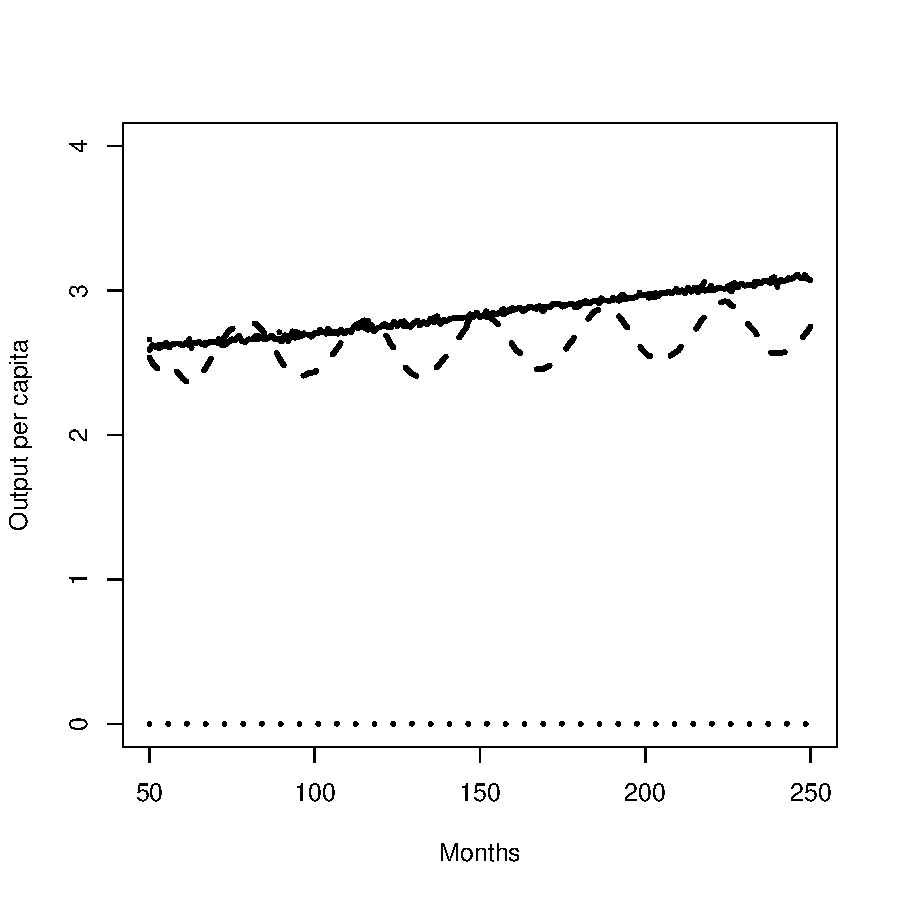
\includegraphics[scale =0.4]{./robustness/gdp_quantil.pdf}
\end{minipage}\hfill
\begin{minipage}[b]{.46\linewidth}
\centering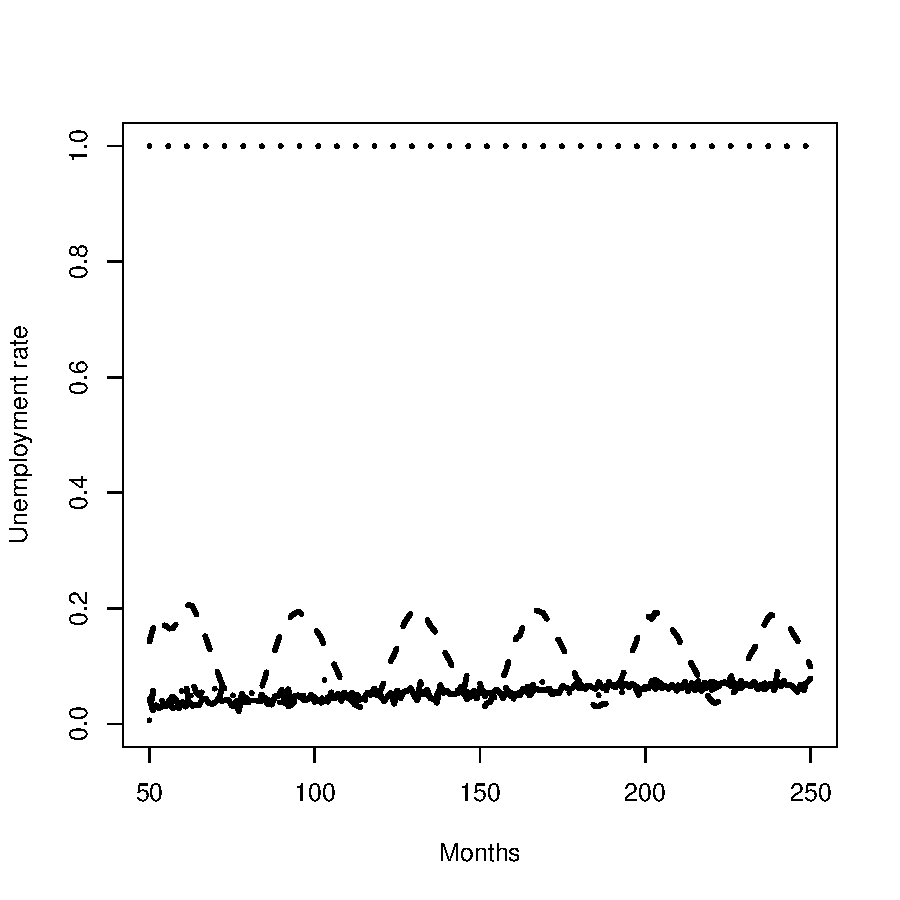
\includegraphics[scale=0.4]{./robustness/unemployment_quantil.pdf}
\end{minipage}
\caption{Sensitivity of the model to a variation in the stock-out probability on output per capita (left panel) and unemployment rate (right panel); 90 \% dotted line, 50\% dashed line, 20\% solid line, and 2.5\% dashed-dotted line.}
\label{parameter_variation}
\end{figure}

\section{Time synchronization}

In the second experiment we test if the time scale on which the agents make their decisions plays any role for the simulation outcome. In the majority of agent-based models there is a strong time-synchronization of actions because all agents make the same type of decisions simultaneously. In EURACE we have two different kinds of triggers for agent's actions: Event driven decisions are made if certain conditions in the agent's environment have changed and is reflected by a change in agent's memory (e.g. if a household becomes unemployed); however, most of the agent's decisions are calendar-time driven. This means there are fixed days in the month (respectively week or year) on which agents take certain actions. For example firms' decision about their monthly production quantities are made on fixed days of the month. These days of the month to act can vary between agents such that we have asynchronized production cycles. In the other case these days coincide such that we have synchronized activation days. The timing of production cycles has a high potential to influence the comparative performance since it sets the day when firms enter the labour, credit, financial and consumption goods market; consequently, this determines whether on all these markets the activities of agents are completely synchronized or not. The EURACE framework allows to explicitly study the aggregate effects of time-synchronization of individual behavior by varying these activation days.  

Figure~\ref{synchron_variation} shows the influence of an asynchronized versus synchronized decision making process of agents on the macroeconomic variables output per capita and unemployment rate. The effect is not that noticeable but especially the impact on the unemployment rate is verifiable. The unemployment is lower when decisions are made asynchroneously.

\begin{figure}[t]
\begin{minipage}[b]{.46\linewidth}
\centering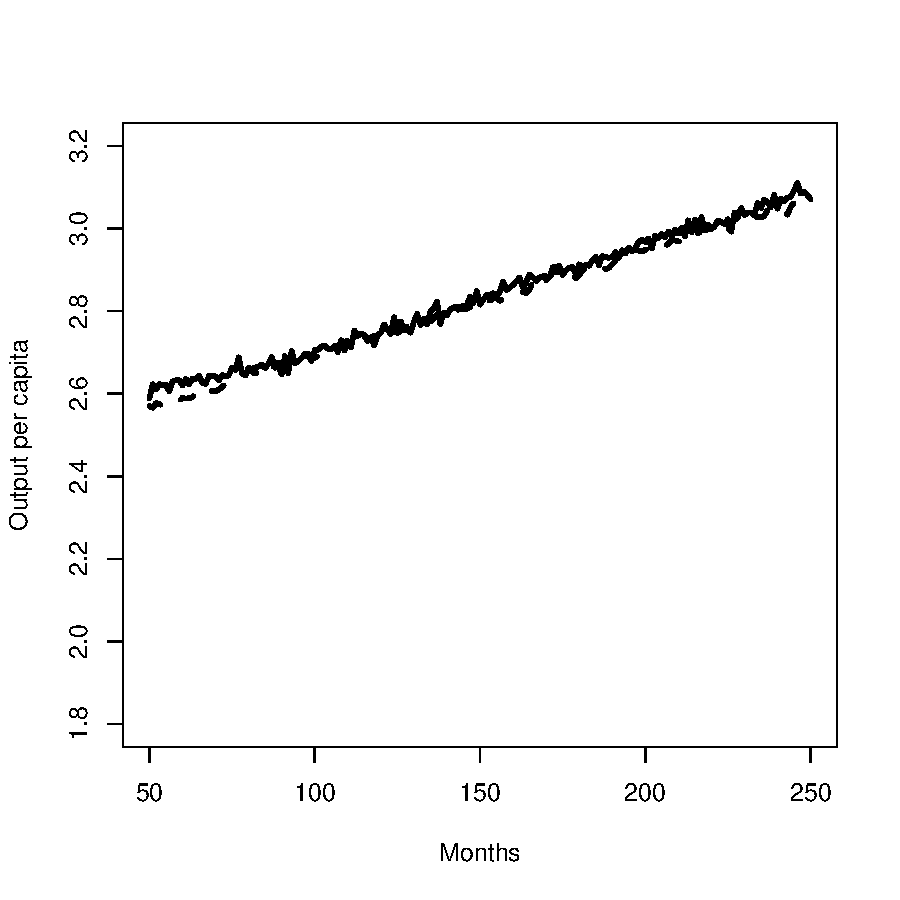
\includegraphics[scale =0.4]{./robustness/gdp_synchron.pdf}
\end{minipage}\hfill
\begin{minipage}[b]{.46\linewidth}
\centering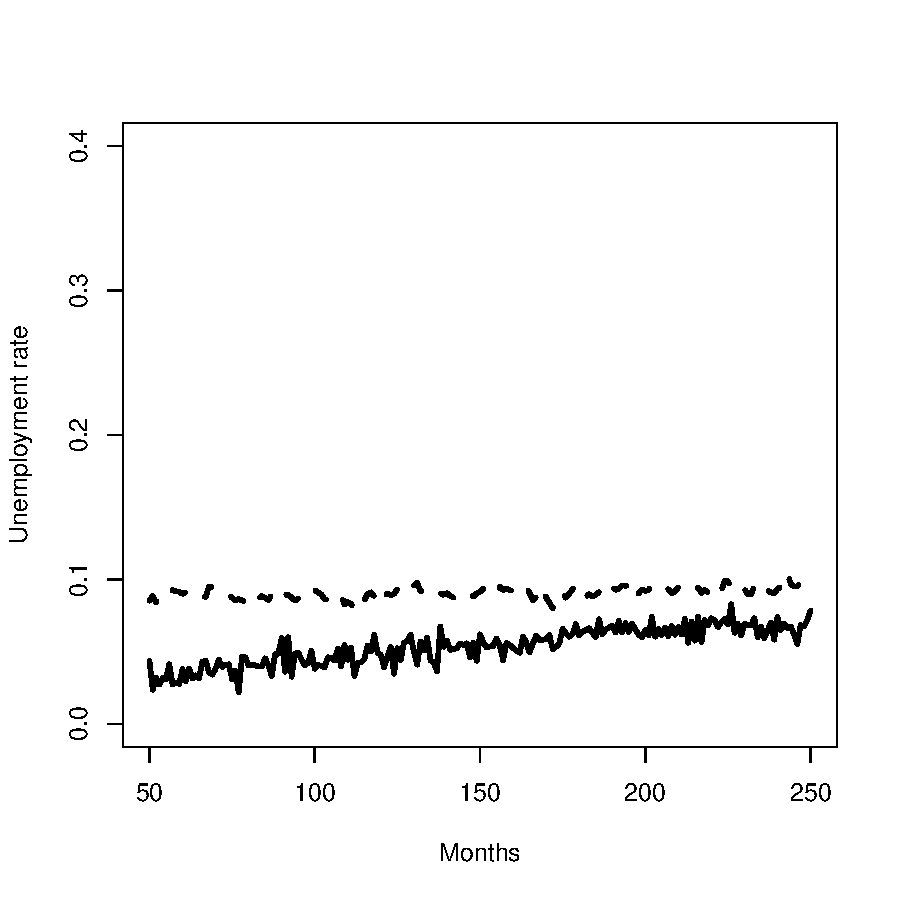
\includegraphics[scale=0.4]{./robustness/unemployment_synchron.pdf}
\end{minipage}
\caption{Differences in output per capita (left panel) and unemployment (right panel) of a asynchronized (solid line) versus synchronized (dashed line) decision making.}
\label{synchron_variation}
\end{figure}

\section{Population scaling}

The third experiment investigates the effect of scaling the population size thereby leaving the ratio between households and firms constant. Furthermore the initial production plan and the firm's endowment with capital and households' with wealth is not changed. 

A priori the impact of the population size is not clear but it should be a very important point of interest when talking about agent-based macroeconomic models. The computational effort to run and analyze large-scale agent-based models is still enormous, and from that perspective the question is still worthwhile if there are additional gains from large-scale simulations in fact. So the question that could be posed is: Is it necessary to run a macro model with an empirically reasonable number of agents or is a small scale model also able to generate the same insights? Note that \cite{Axtell_2000} makes the point that in order to reproduce the firm size distribution one needs at least several millions of workers, since empirically the largest firm (Wall Mart) has 1.5 million employees, and there are one million companies with one worker (self employed).     

Figure~\ref{scaling_variation} indicates that the EURACE model is very robust against a variation of the population size. In terms of output per capita there is just a small difference that establishes after month 150 (iteration 3000), where a scaling effect on the unemployment rate is not detectable. Thus, this final experiment pointed to the robustness against an increase in the number of agents in absolute terms where their relative number as well as the initial conditions are kept unchanged. 

This experiment suggests that the additional advantage seems to be small and a reasonable analysis of an agent-based macro model can be based on small scale models. In any case, this experiment was run with a maximum number of 10.000 households, far away from the empirical number of households in a real economy. 

A low sensitivity to a population scaling is true for the given model set up. The model used for these tests has only one region and all agents have the identical initial conditions. If the model is more refined in the sense that it is set up with more than one region and the initial memory of agents is set according to empirical distributions the population size might matter.  

\begin{figure}[t]
\begin{minipage}[b]{.46\linewidth}
\centering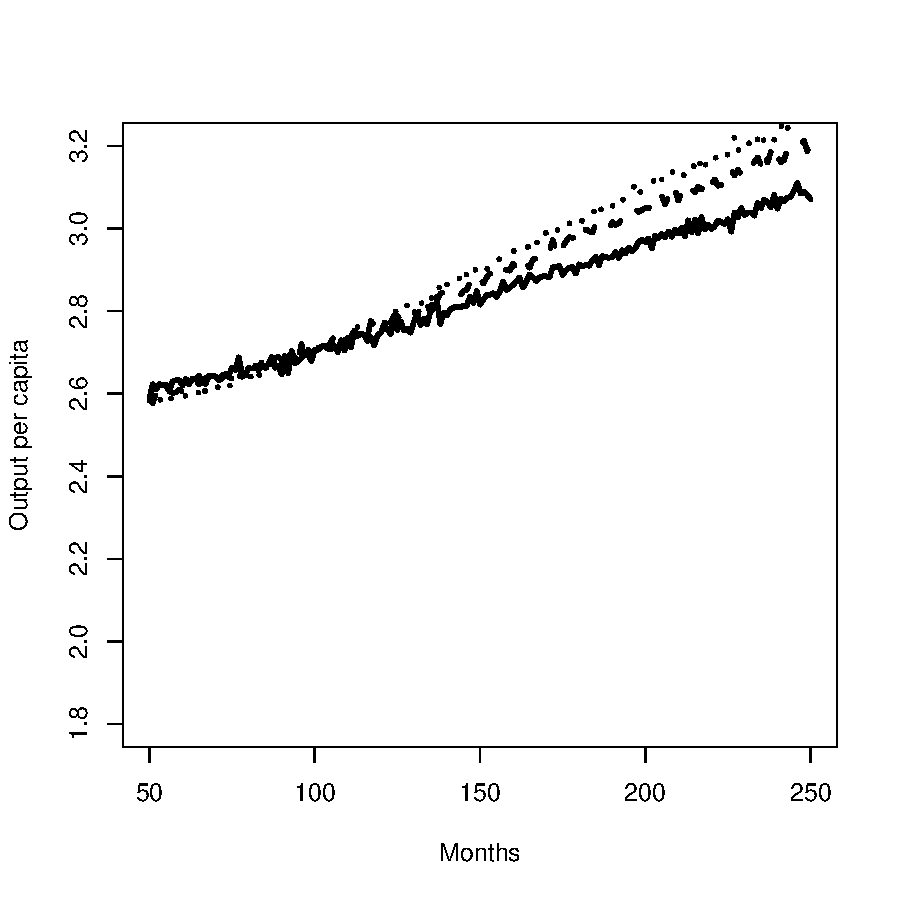
\includegraphics[scale =0.4]{./robustness/gdp_scaling.pdf}
\end{minipage}\hfill
\begin{minipage}[b]{.46\linewidth}
\centering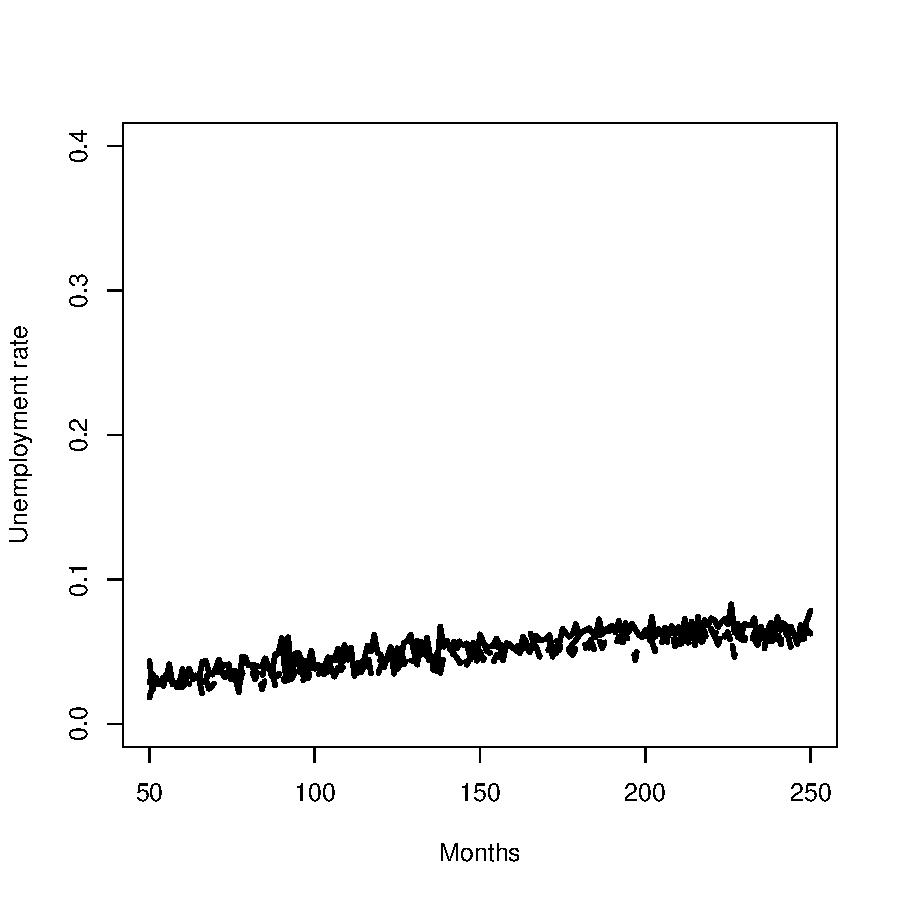
\includegraphics[scale=0.4]{./robustness/unemployment_scaling.pdf}
\end{minipage}
\caption{Impact of scaling of the agent population on aggregate output and unemployment; solid line 1600 households and 80 firms, dashed line 5000/250, and dotted line 10.000/500.}
\label{scaling_variation}
\end{figure}


\chapter{Benchmark simulations with the EURACE Model}
\section{Transient period}
Before we show the benchmark results, we show a transient run for the default parameter settings.
Figure \ref{Figure: transient time} shows a simulation of the model for $20$ batch runs of $5000$ iterations.
After approximately $1000$ iterations the transient phase settles down to stochastic steady state.

The data is summarized using a box-and-whisker plot in which the dark grey area shows the data between Q1 and Q3 ($50\%$ of the data) and
 the light grey area indicates the outer hinges of the distribution, i.e. $1.5$ times the interquartile range (IQR).
In Figure \ref{Figure: run batch} the box plots show the distribution for each single run.

\bigskip
The main features of the benchmark runs are:
\begin{itemize}
\item GDP converges to a level of $1300$ and then sets off on a stable growth path.
\item The unemployment rate approaches a stable level of $30\%$.
\item Inflation rates are between $-5\%$ and $+5\%$ for most periods,
although in some periods inflation rates of $-20\%$ and $+20\%$ can occur.
\item The investment/GDP ratio fluctuates around $15\%$.
\end{itemize}

\section{Benchmark scenario}
In this section we show a more detailed overview of the economy that will serve as our benchmark scenario.
We show cross sectional data across the various sectors of the economy (Consumption goods, Investment goods, Credit market),
and for the different types of agents (Firms, Banks, Households, Government). 

Of course there is always a danger of showing too many plots and too much data,
but it appears to us essential to do this exercise one time and to show the reader how
all the elements of the EURACE system fit together.

In this and all following sections we omit the transient phase of $1000$ periods and only show results for iterations $1001-5000$.
All plots show distributional data for $20$ batch runs. The results reported here are for an income tax rate of $10\%$.

\subsubsection*{Macrodata}
We have already shown the general trends pertaining to the macroeconomic data in Figure \ref{Figure: transient time} above. 
In Figure \ref{Figure: Eurostat macrodata growth rates} we show the growth rates of GDP, monthly output, the unemployment rate, and the average wage.

The growth rates of the benchmark runs are:
\begin{itemize}
\item The GDP growth rate is about $3$ to $4\%$ annually.
\item The output growth rate is approx. $4\%$.
\item The average wage grows $3\%$ per year.
\end{itemize}

\subsubsection*{Government}
For the Government financing we show in Figure \ref{Figure: Government} the monthly tax revenues, total benefit payments, the monthly budget balance,
and the total amount of bond financing.

The growth rate of tax revenues and of benefit payments are approximately equal, but
since the level of tax revenues is lower than that of the unemployment benefit payout there is a monthly budget deficit.
This deficit needs to be financed by government bonds, as showns in Fig. \ref{Figure: Government}d.

\subsubsection*{Firms}
For the firms we show in Figure \ref{Figure: Firm Production} the monthly output, cumulative revenues, number of employees, the actual capital price paid for machinery, and the firm's payment account. The average firm size measured by the number of employees is $25$.

The earnings data and the cumulative revenues show a wide distribution. To show that this is not due to one or two special runs but a general feature of all runs, we  show in Figure \ref{Figure: Firm Production batch} the complete set of batch run box plots. This plot makes clear that in each run the population distribution of the firms' earnings and cumulative revenues is wide.
Whether or not the earnings distribution has power law tails we have not yet investigated.

The firms' financial data are shown in Figure \ref{Figure: Firm Financial Data}. We show total assets, debt and equity, as well as
the average debt earnings ratio and the average debt equity ratio (first averaged across firms, then averaged across runs).

Total assets increase, while total debt decreases, so equity is increased. Total earnings stabilize to a level of 50.
The debt earnings ratios and the debt equity ratios decrease asymptotically to 0 since debt decreases.

\subsubsection*{Labour market}
From the labour market data we show the average unemployment rate, the unemployment rate for skill level 1 and 5, the average wage and 
average wage for skill level 1 and 5. Next we show the total number of vacancies and the labour/profit share ratio.

Figure \ref{Figure: Labour Market} shows that the unemployment rate stabilizes to $32\%$, but due to the heteregeneity in workers' skill level there are stark differences: the unemployment rate for skill level 1 is $56\%$ while for skill level  5 it is $14\%$.

Figure \ref{Figure: Labour Market 2} shows that the average labour share ratio converges to 3, which means that the total wage bill is 3 times the profits.

\subsubsection*{Consumption Goods Market}
From the consumption goods market we show data pertaining to: monthly output, monthly planned output, quantity sold, total monthly revenues,
the firms' average productivity, and the firms' average productivity progress (see Fig. \ref{Figure: Consumption Market}). This should give a good idea of the production sector.
All data are steadily increasing with the average productivity progress of $2.5\%$.

\subsubsection*{Credit Market}
There are two banks in the system. 
We show the banks' cash, total deposits, the total credit given to firms, bank equity, ECB debt, and the banks' total dividend payout.
On the credit market we see in Figure \ref{Figure: Credit Market} that banks deposits are increasing, total credits to firms are converging to a constant level, and banks' equity is increasing as well. Furthermore, banks have no ECB debt, and are able to pay out positive dividends to the households.


\section{Tax rate scenarios}
In a first sensitivity analysis we consider three income tax rate scenarios, using respectively a $5\%$, $10\%$ and $15\%$ income tax.

In Figure \ref{Figure: scenarios} we show results for GDP, the unemployment rate and the investment/GDP ratio.
It is clear that if we increase the tax rate the GDP decreases and unemployment increases.
The investment/GDP ratio remains constant which means that total investments in the economy show the same decrease as GDP when the tax rate is increased.

%%%%%%%%%%%%%%% Include all figures
%\subsubsection*{Transient}

\begin{figure}[ht!]
\centering\leavevmode
\begin{minipage}{17cm}
\centering\leavevmode
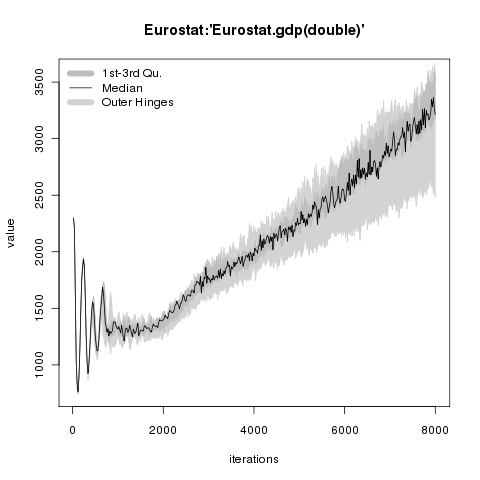
\includegraphics[width=8cm]{./transient/tax_0.08/Eurostat-gdp.png}
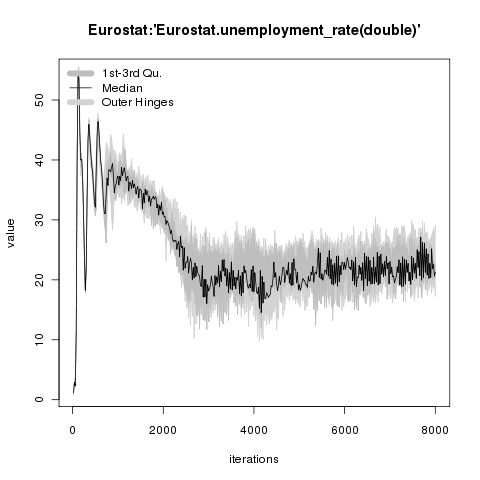
\includegraphics[width=8cm]{./transient/tax_0.08/Eurostat-unemployment_rate.png}\\
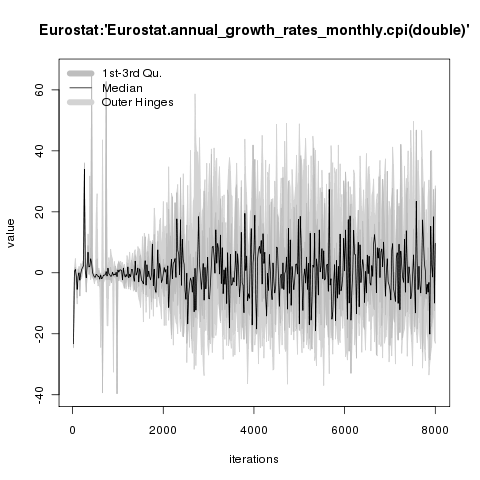
\includegraphics[width=8cm]{./transient/tax_0.08/Eurostat-cpi.png}
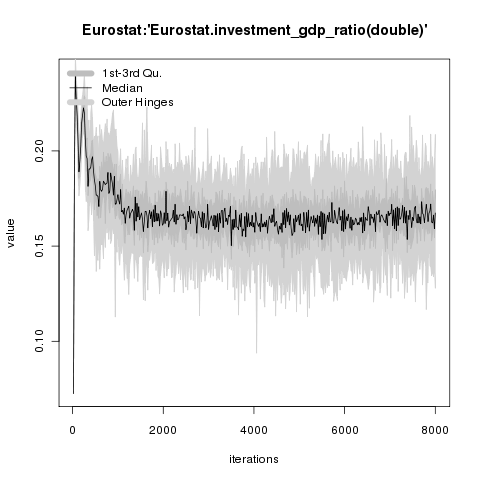
\includegraphics[width=8cm]{./transient/tax_0.08/Eurostat-investment_gdp_ratio.png}
\end{minipage}
\caption{Time series plots for 20 batch runs. GDP, unemployment rate, inflation rate and investment/GDP ratio.}
\label{Figure: transient time}
\end{figure}

%\subsubsection*{Distribution across batch runs}

\begin{figure}[ht!]
\centering\leavevmode
\begin{minipage}{17cm}
\centering\leavevmode
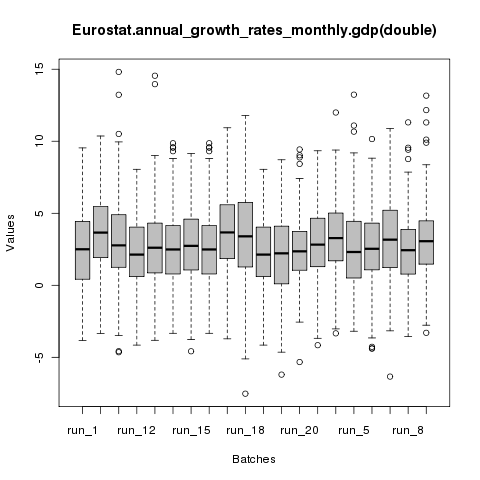
\includegraphics[width=8cm]{./benchmark_plots/Eurostat-annual_growth_rates_monthly-gdp-batches.png}
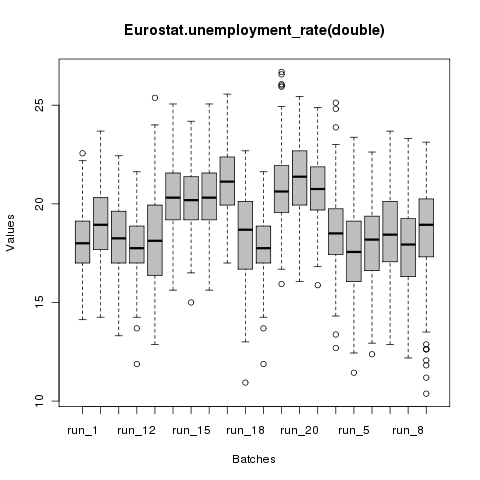
\includegraphics[width=8cm]{./benchmark_plots/Eurostat-unemployment_rate-batches.png}\\
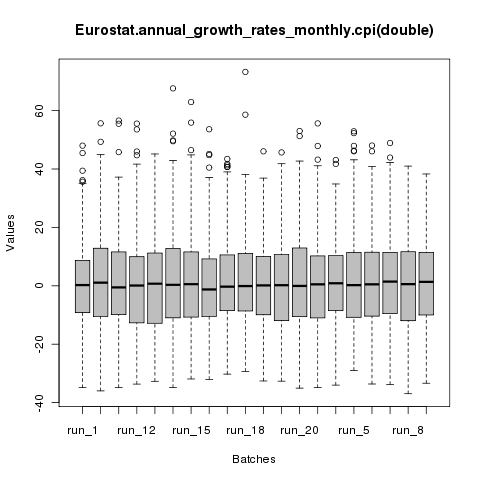
\includegraphics[width=8cm]{./benchmark_plots/Eurostat-cpi-batches.png}
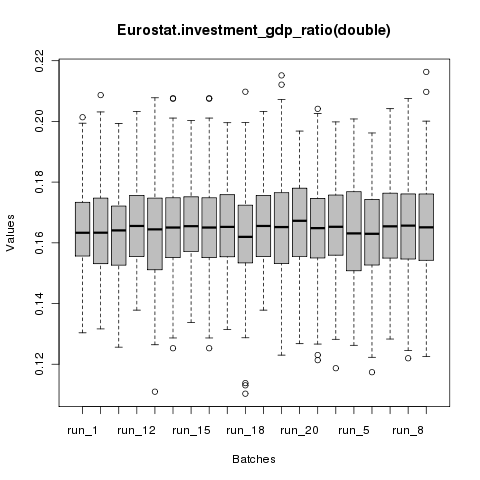
\includegraphics[width=8cm]{./benchmark_plots/Eurostat-investment_gdp_ratio-batches.png}
\end{minipage}
\caption{Box plots for separate runs of GDP, unemployment rate, inflation rate and investment/GDP ratio.}
\label{Figure: run batch}
\end{figure}

\begin{comment}
\documentclass{article}
\usepackage{epsfig,graphicx,verbatim, boxedminipage, url}
\begin{document}
\end{comment}

\begin{comment}
%\subsubsection*{Eurostat macrodata}
\begin{figure}[H!]
\centering\leavevmode
\begin{minipage}{14cm}
\centering\leavevmode
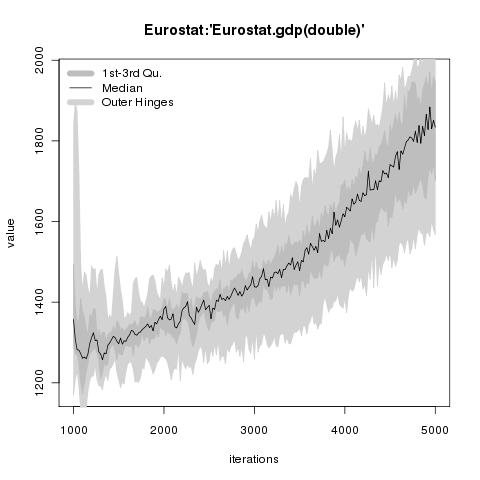
\includegraphics[width=6cm]{./png/tax_0.10/Eurostat-gdp.png}
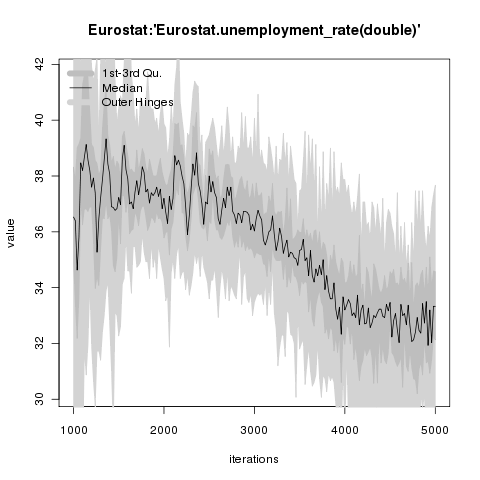
\includegraphics[width=6cm]{./png/tax_0.10/Eurostat-unemployment_rate.png}
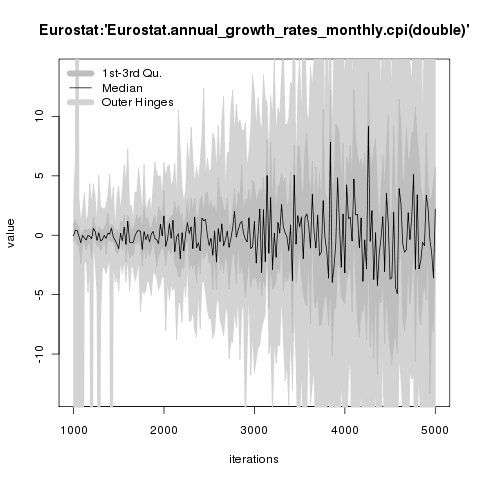
\includegraphics[width=6cm]{./png/tax_0.10/Eurostat-annual_growth_rates_monthly_cpi.png}
\end{minipage}
\caption{Eurostat: GDP, unemployment rate and inflation rate (annual, measured monthly).}
\label{Figure: Eurostat macrodata}
\end{figure}
\end{comment}

%\begin{comment}
%\subsubsection*{Growth rates}
\begin{figure}[H!]
\centering\leavevmode
\begin{minipage}{14cm}
\centering\leavevmode
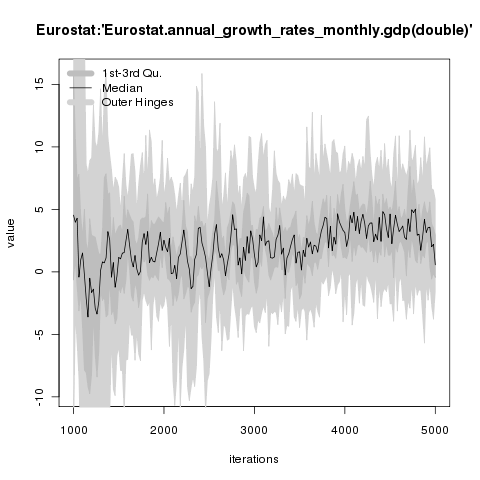
\includegraphics[width=6cm]{./png/tax_0.10/Eurostat-annual_growth_rates_monthly_gdp.png}
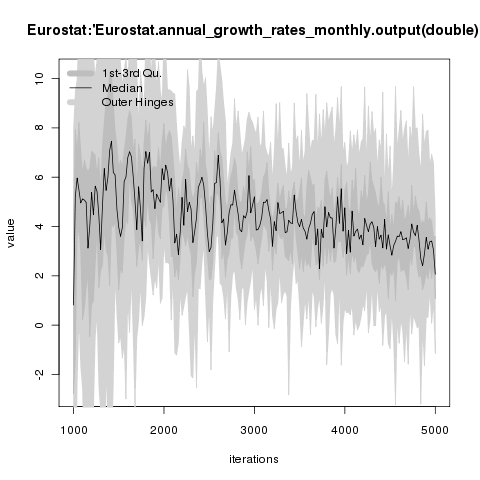
\includegraphics[width=6cm]{./png/tax_0.10/Eurostat-annual_growth_rates_monthly_output.png}\\
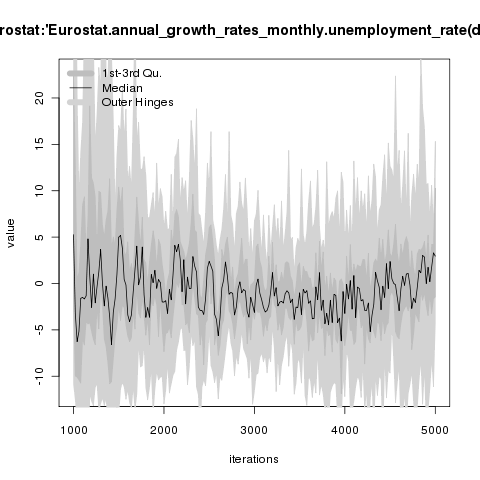
\includegraphics[width=6cm]{./png/tax_0.10/Eurostat-annual_growth_rates_monthly_unemployment_rate.png}
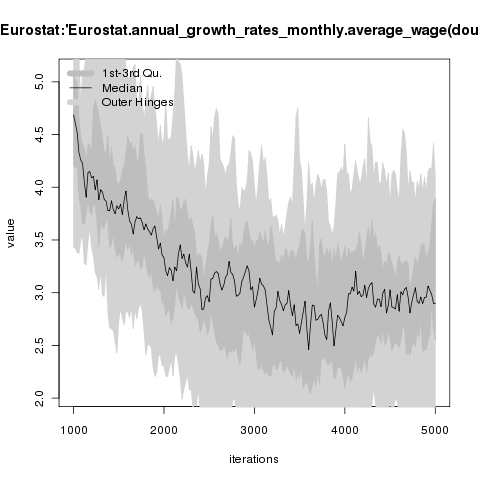
\includegraphics[width=6cm]{./png/tax_0.10/Eurostat-annual_growth_rates_monthly_average_wage.png}
\end{minipage}
\caption{Annual growth rates (with respect to same month in the previous year): GDP, output, unemployment rate and avgerage wage. Tax: $10\%$.}
\label{Figure: Eurostat macrodata growth rates}
\end{figure}
\clearpage
%\end{comment}

%\pagebreak
%\subsubsection*{Government}
\begin{figure}[H!]
\centering\leavevmode
\begin{minipage}{14cm}
\centering\leavevmode
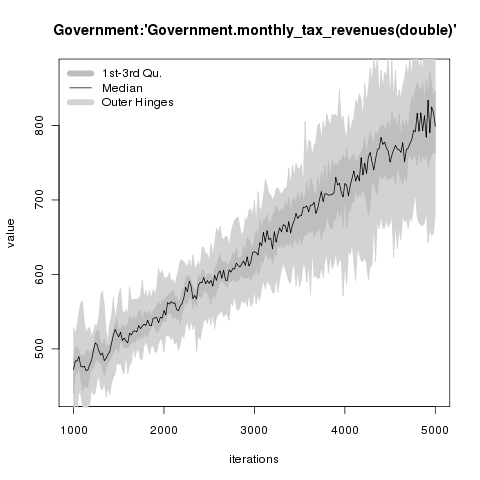
\includegraphics[width=6cm]{./png/tax_0.10/Government-monthly_tax_revenues.png}
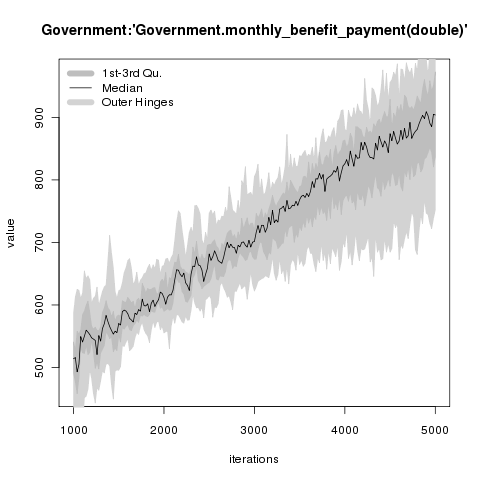
\includegraphics[width=6cm]{./png/tax_0.10/Government-monthly_benefit_payment.png}\\
%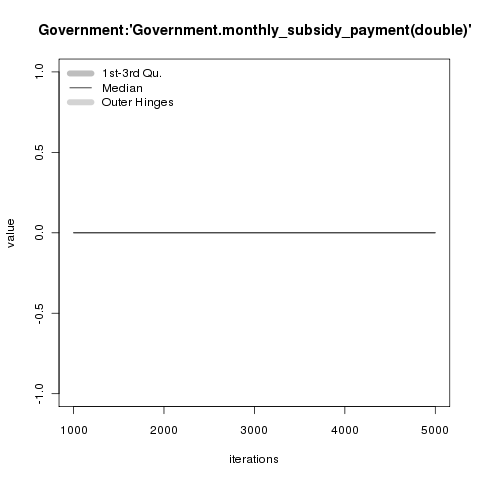
\includegraphics[width=6cm]{./png/tax_0.10/Government-monthly_subsidy_payment.png}
%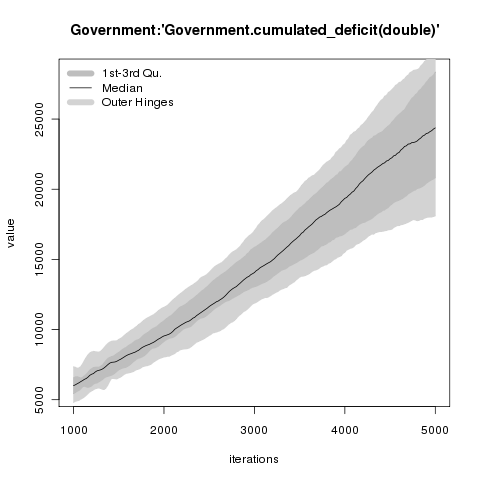
\includegraphics[width=6cm]{./png/tax_0.10/Government-cumulated_deficit.png}
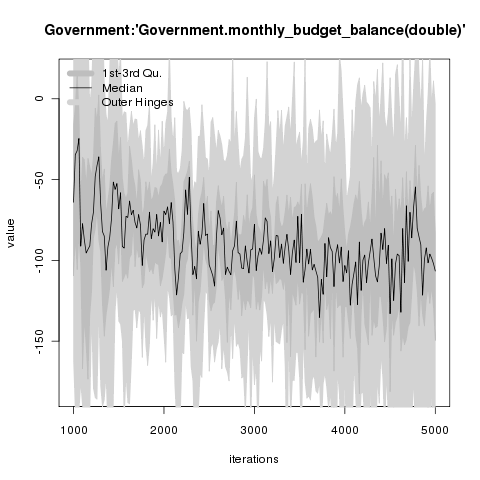
\includegraphics[width=6cm]{./png/tax_0.10/Government-monthly_budget_balance.png}
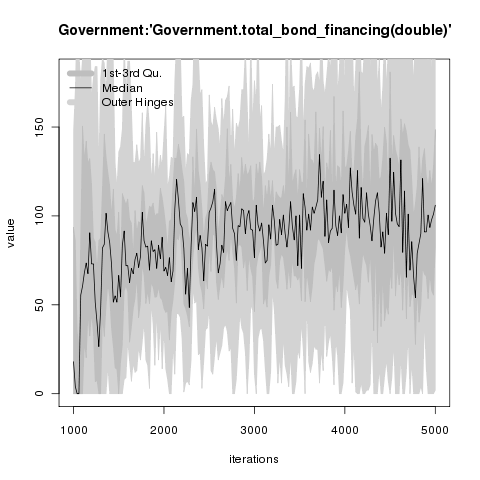
\includegraphics[width=6cm]{./png/tax_0.10/Government-total_bond_financing.png}
%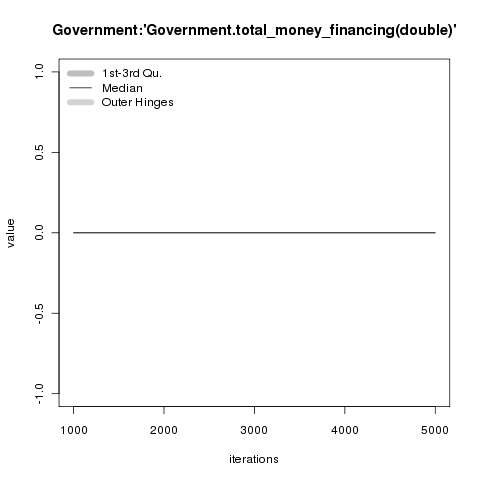
\includegraphics[width=6cm]{./png/tax_0.10/Government-total_money_financing.png}
\end{minipage}
\caption{Government finances.}
\label{Figure: Government}
\end{figure}
\clearpage

%\pagebreak
%\subsubsection*{Firms}
\begin{figure}[H!]
\centering\leavevmode
\begin{minipage}{14cm}
\centering\leavevmode
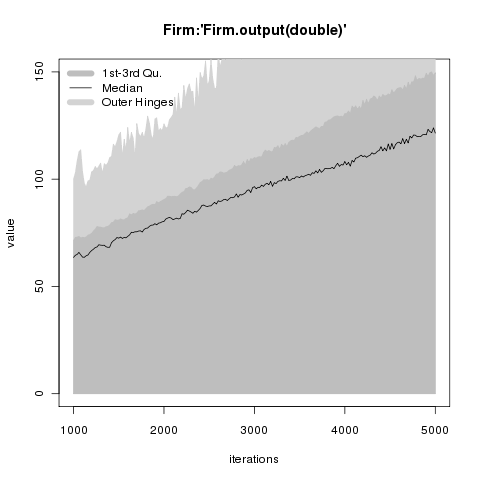
\includegraphics[width=6cm]{./png/tax_0.10/Firm-output.png}
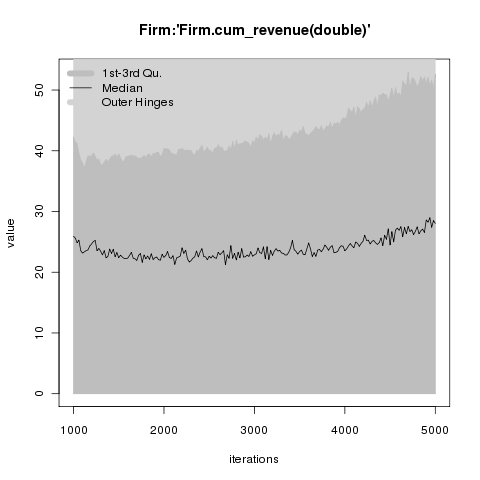
\includegraphics[width=6cm]{./png/tax_0.10/Firm-cum_revenue.png}\\
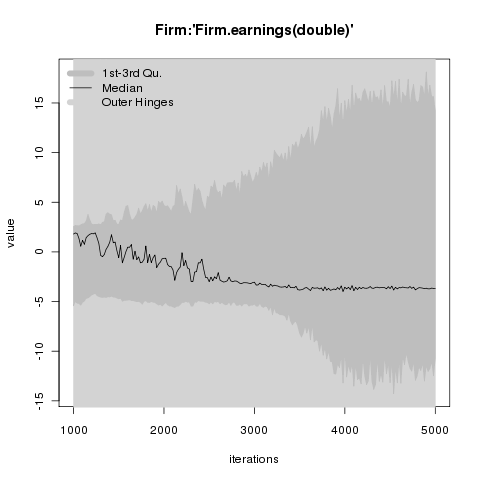
\includegraphics[width=6cm]{./png/tax_0.10/Firm-earnings.png}
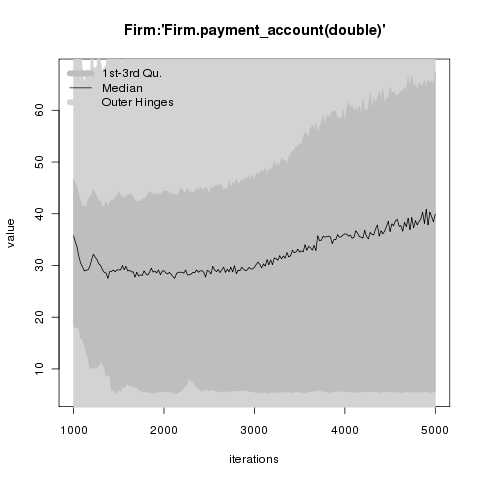
\includegraphics[width=6cm]{./png/tax_0.10/Firm-payment_account.png}\\
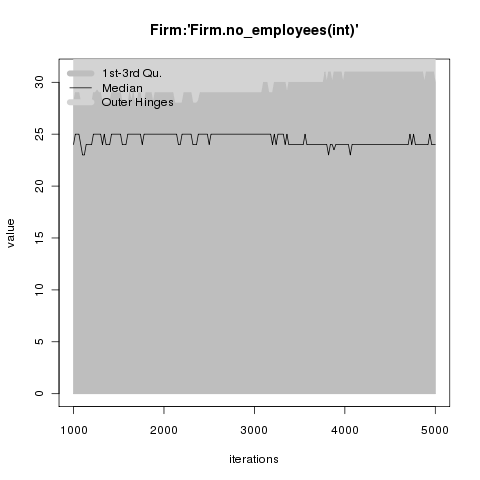
\includegraphics[width=6cm]{./png/tax_0.10/Firm-no_employees.png}
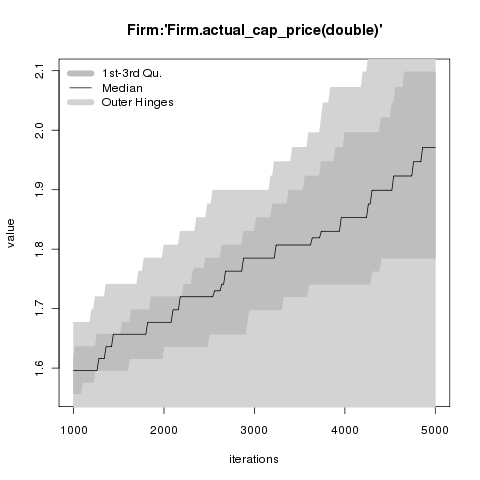
\includegraphics[width=6cm]{./png/tax_0.10/Firm-actual_cap_price.png}
%\includegraphics[width=6cm]{./png/tax_0.10/Firm-bankruptcy_state.png}
\end{minipage}
\caption{Firm production data.}
\label{Figure: Firm Production}
\end{figure}

\begin{figure}[H!]
\centering\leavevmode
\begin{minipage}{14cm}
\centering\leavevmode
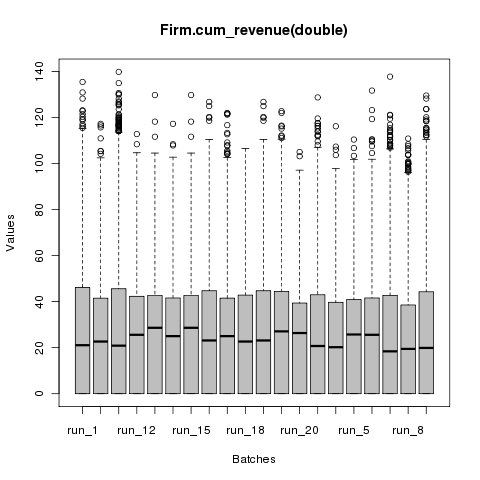
\includegraphics[width=6cm]{./png/tax_0.10/Firm-cum_revenue-batches.png}
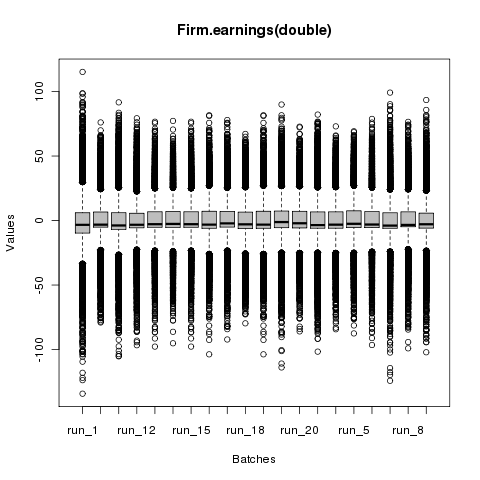
\includegraphics[width=6cm]{./png/tax_0.10/Firm-earnings-batches.png}
\end{minipage}
\caption{Firm production data, all batch runs.}
\label{Figure: Firm Production batch}
\end{figure}
\clearpage


%\subsubsection*{Financial Data}
\begin{figure}[H!]
\centering\leavevmode
\begin{minipage}{14cm}
\centering\leavevmode
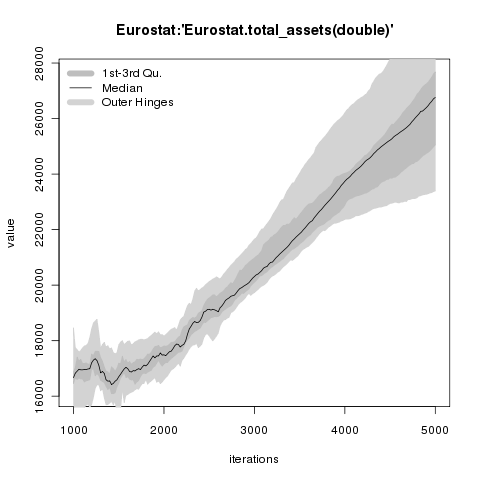
\includegraphics[width=6cm]{./png/tax_0.10/Eurostat-total_assets.png}
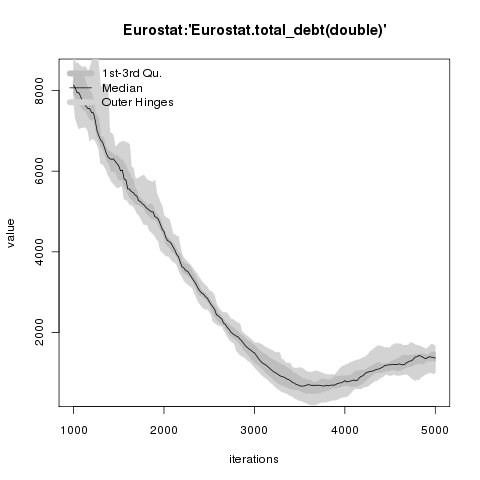
\includegraphics[width=6cm]{./png/tax_0.10/Eurostat-total_debt.png}\\
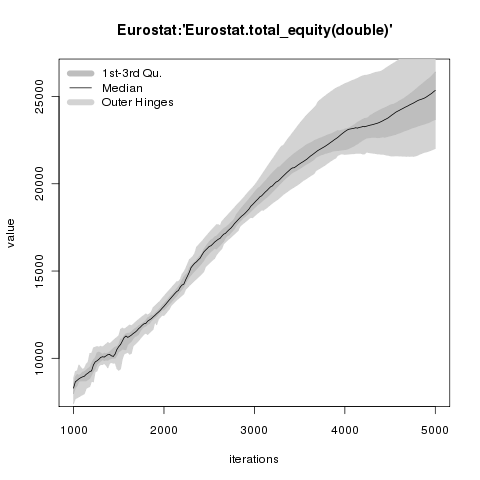
\includegraphics[width=6cm]{./png/tax_0.10/Eurostat-total_equity.png}
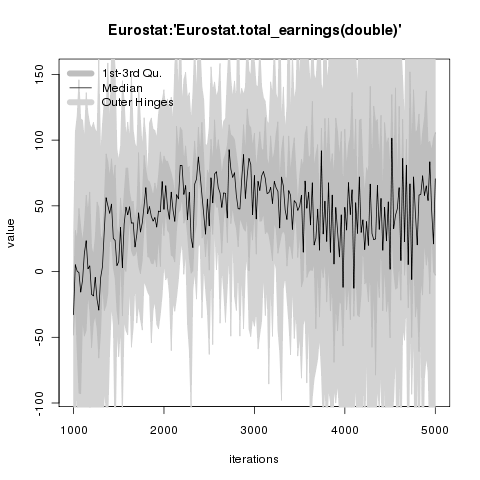
\includegraphics[width=6cm]{./png/tax_0.10/Eurostat-total_earnings.png}\\
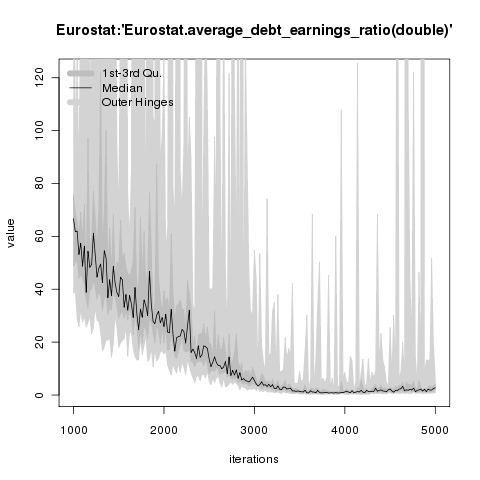
\includegraphics[width=6cm]{./png/tax_0.10/Eurostat-average_debt_earnings_ratio.png}
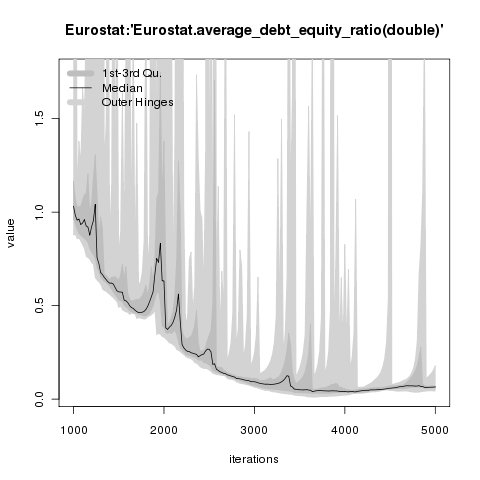
\includegraphics[width=6cm]{./png/tax_0.10/Eurostat-average_debt_equity_ratio.png}
\end{minipage}
\caption{Firm financial data.}
\label{Figure: Firm Financial Data}
\end{figure}


%\pagebreak
%\subsubsection*{Labour Market}
\begin{figure}[H!]
\centering\leavevmode
\begin{minipage}{14cm}
\centering\leavevmode
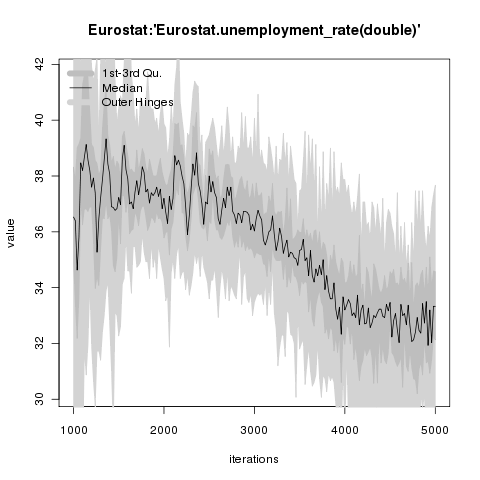
\includegraphics[width=6cm]{./png/tax_0.10/Eurostat-unemployment_rate.png}
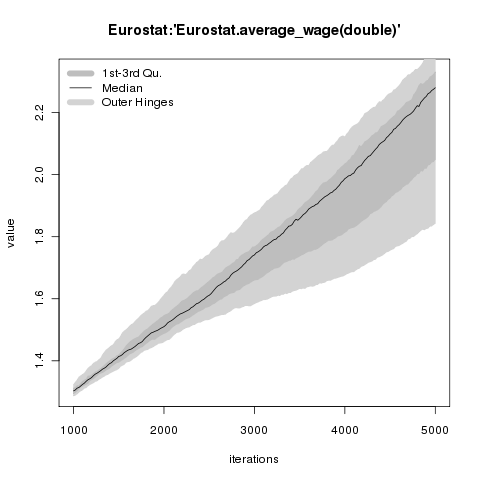
\includegraphics[width=6cm]{./png/tax_0.10/Eurostat-average_wage.png}\\
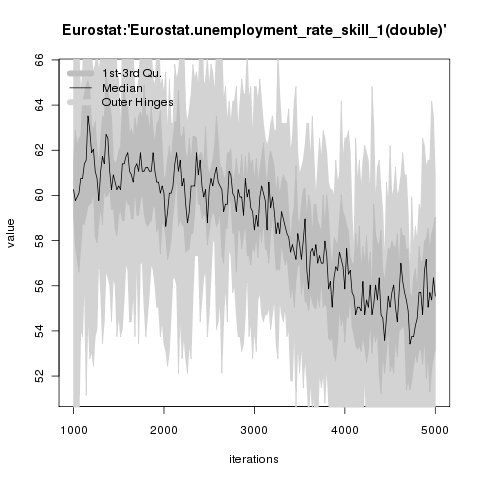
\includegraphics[width=6cm]{./png/tax_0.10/Eurostat-unemployment_rate_skill_1.png}
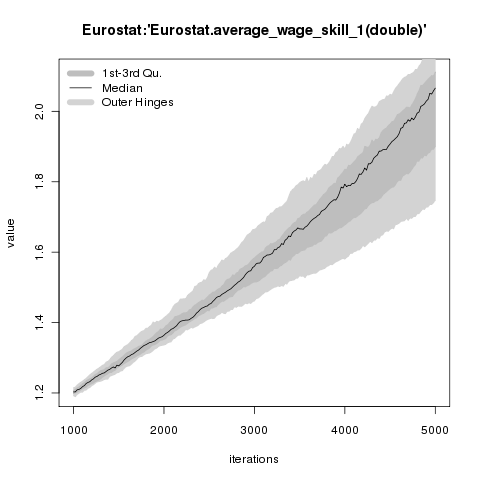
\includegraphics[width=6cm]{./png/tax_0.10/Eurostat-average_wage_skill_1.png}\\
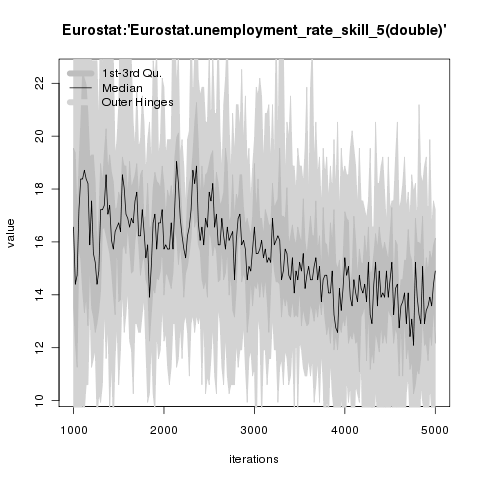
\includegraphics[width=6cm]{./png/tax_0.10/Eurostat-unemployment_rate_skill_5.png}
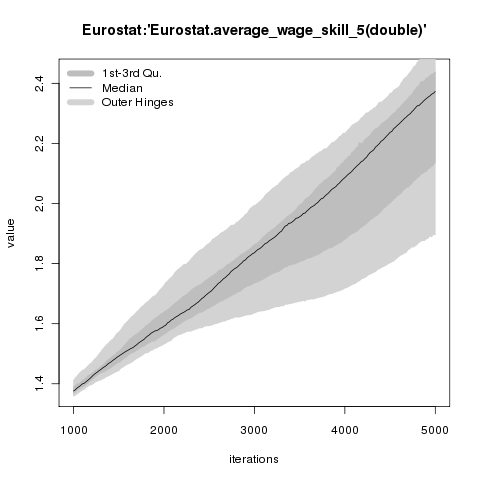
\includegraphics[width=6cm]{./png/tax_0.10/Eurostat-average_wage_skill_5.png}
\end{minipage}
\caption{Labour market data.}
\label{Figure: Labour Market}
\end{figure}


\begin{figure}[H!]
\centering\leavevmode
\begin{minipage}{14cm}
\centering\leavevmode
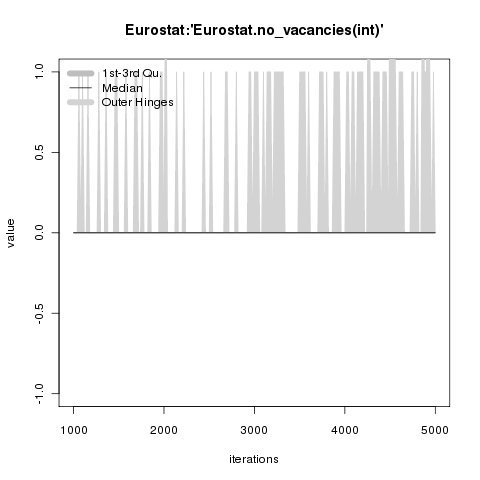
\includegraphics[width=6cm]{./png/tax_0.10/Eurostat-no_vacancies.png}
\includegraphics[width=6cm]{./png/tax_0.10/Eurostat-labour_share_ratio.png}\\
\includegraphics[width=6cm]{./png/tax_0.10/Eurostat-average_s_skill.png}
\end{minipage}
\caption{Labour market data (cont).}
\label{Figure: Labour Market 2}
\end{figure}

\clearpage


%\subsubsection*{Consumption Market}
\begin{figure}[H!]
\centering\leavevmode
\begin{minipage}{14cm}
\centering\leavevmode
\includegraphics[width=6cm]{./png/tax_0.10/Eurostat-monthly_output.png}
\includegraphics[width=6cm]{./png/tax_0.10/Eurostat-monthly_planned_output.png}\\
\includegraphics[width=6cm]{./png/tax_0.10/Eurostat-monthly_sold_quantity.png}
\includegraphics[width=6cm]{./png/tax_0.10/Eurostat-monthly_revenue.png}\\
\includegraphics[width=6cm]{./png/tax_0.10/Eurostat-firm_average_productivity.png}
\includegraphics[width=6cm]{./png/tax_0.10/Eurostat-firm_average_productivity_progress.png}
\end{minipage}
\caption{Consumption goods market.}
\label{Figure: Consumption Market}
\end{figure}
\clearpage


%\pagebreak
%\subsubsection*{Credit market}
\begin{figure}[H!]
\centering\leavevmode
\begin{minipage}{14cm}
\centering\leavevmode
\includegraphics[width=6cm]{./png/tax_0.10/Bank-cash.png}
\includegraphics[width=6cm]{./png/tax_0.10/Bank-deposits.png}\\
\includegraphics[width=6cm]{./png/tax_0.10/Bank-total_credit.png}
\includegraphics[width=6cm]{./png/tax_0.10/Bank-equity.png}\\
\includegraphics[width=6cm]{./png/tax_0.10/Bank-ecb_debt.png}
\includegraphics[width=6cm]{./png/tax_0.10/Bank-total_dividends.png}
\end{minipage}
\caption{Credit market data.}
\label{Figure: Credit Market}
\end{figure}
%\clearpage

%\end{document}

\begin{figure}[ht!]
\centering\leavevmode
\begin{minipage}{7.5cm}
\centering\leavevmode
\includegraphics[width=6cm]{./batch/Eurostat-annual_growth_rates_monthly-gdp-scenarios.png}\\
\includegraphics[width=6cm]{./batch/Eurostat-unemployment_rate-scenarios.png}\\
\includegraphics[width=6cm]{./batch/Eurostat-investment_gdp_ratio-scenarios.png}
\end{minipage}
\caption{Parameter sensitivity analysis for different tax rates of $0-8\%$ and $10,15,20\%$. Results are for $20$ batch runs over $4000$ periods (using periods $4001$ to $8000$).}
\label{Figure: scenarios}
\end{figure}




\begin{appendix}
\chapter{Model parameters}
In Table \ref{Table: constants} we provide a listing of all the model parameters.

\begin{landscape}
\begin{longtable}[H!]{lll}
\caption{{\bfseries List of parameters.}}
\label{Table: constants}\\
\toprule 
\bfseries Name & \bfseries Value & \bfseries Description \\ \hline 
\midrule
\endfirsthead
\multicolumn{3}{c}%
{{\bfseries \tablename\ \thetable{} -- continued from previous page}} \\
\toprule
\bfseries Name & \bfseries Value & \bfseries Description \\ \hline 
\midrule
\endhead
\multicolumn{3}{r}{{\emph{Continued on next page}}} \\
\endfoot
\bottomrule
\endlastfoot
\url{int} \url{total_regions} & 1 & \parbox{10cm}{Total number of regions.}\\
\url{int} \url{const_bankruptcy_idle_period} & 240 & \parbox{10cm}{Number of iterations that a bankrupt firm remains idle, before resuming production activity.}\\
\url{int} \url{days_per_month} & 20 & \parbox{10cm}{Optional setting for the number of days in a month.}\\
\url{int} \url{number_of_banks_to_apply} & 2 & \parbox{10cm}{Number of banks to which firms can apply for loans.}\\
\url{int} \url{const_number_of_banks} & 2 & \parbox{10cm}{Total number of banks.}\\
\url{int} \url{const_installment_periods} & 24 & \parbox{10cm}{Number of months to make debt installment payments before a loan is fully repaid.}\\
\url{double} \url{const_wage_wealth_ratio} & 0.2 & \parbox{10cm}{The household's initial ratio between wage and wealth. This parametrizes the link between the unit price of capital and the unit price of labour.}\\
\url{double} \url{const_firm_leverage} & 2 & \parbox{10cm}{Initial leverage (debt/equity ratio) of each firm.}\\
\url{double} \url{const_income_tax_rate} & 0.2 & \parbox{10cm}{Constant income tax rate for sensitivity analysis.}\\
\url{double} \url{debt_rescaling_factor} & 0.8 & \parbox{10cm}{The debt rescaling factor $\omega$ is used in case of a firm bankruptcy to rescale the debt. This is a process of debt-to-equity transformation. It sets the target debt level in relation to the value of total assets: $L^*=\omega A^*$. The firm will not refund all of its loans completely, but will write off every loan with a certain ratio: $w\_j = (1-L^*/L)L\_j$ for loan $j$. The fraction $(1-L^*/L)$ is the write-off ratio, and $w\_j$ is the monetary amount of the write-off for loan $j$.}\\
\url{double} \url{target_leverage_ratio} & 2 & \parbox{10cm}{The target leverage ratio is the proportion of the target debt to target equity: $\ell = L^*/E^*$. This determines the target equity level as $E^*= (1/\ell) L^*$ and sets the amount of equity that the firm should raise on the financial market.}\\
\url{double} \url{target_liquidity_ratio} & 1.5 & \parbox{10cm}{The target liquidity ratio is a parameter used in the case of firm bankruptcy due to illiquidity. The amount of equity to raise on the AFM equals $\alpha (F-P)$, where $\alpha$ is the target liquidity ratio, F are the financial commitments, and P is the payment account.}\\
\url{double} \url{const_dividend_earnings_ratio} & 0.1 & \parbox{10cm}{The parameter const\_dividend\_earnings\_ratio is used to determine the first positive dividend payment (if the dividend was set to 0, or at the start): TOTAL\_DIVIDEND\_PAYMENT = CONST\_DIVIDEND\_EARNINGS\_RATIO *NET\_EARNINGS;}\\
\url{double} \url{trading_activity} & 0.01 & \parbox{10cm}{household choose randomly to trade or not.}\\
\url{double} \url{bonds_newissue_discount} & 0 & \parbox{10cm}{}\\
\url{int} \url{couponperiodicitynrmonths} & 1 & \parbox{10cm}{payment coupon period expressed in number of months: typical value is 6 }\\
\url{double} \url{fundamental_return_weight_min} & 0.1 & \parbox{10cm}{constant value that regulate the minumum value of the fundamental weight:typical value is 0.1}\\
\url{int} \url{days_in_month} & 20 & \parbox{10cm}{number of days in month : typical value is 20}\\
\url{int} \url{symmetric_shock} & 0 & \parbox{10cm}{Binary parameter to set if the energy shock is symmetric.}\\
\url{int} \url{energy_shock_start} & 0 & \parbox{10cm}{Day when the energy shock starts.}\\
\url{int} \url{energy_shock_end} & 0 & \parbox{10cm}{Day when the energy shock ends.}\\
\url{double} \url{const_energy_shock_intensity} & 0 & \parbox{10cm}{Mark up on the capital goods price that flows out of the system, representing energy costs.}\\
\url{int} \url{energy_shock_frequency} & 0 & \parbox{10cm}{The frequency at which the energy price is updated.}\\
\url{double} \url{gamma_const} & -6.5 & \parbox{10cm}{ -2, Strength of logit rule for consumption}\\
\url{double} \url{alpha} & 0.668 & \parbox{10cm}{0.662, Parameter for production function.}\\
\url{double} \url{beta} & 0.332 & \parbox{10cm}{0.338, Parameter for production function.}\\
\url{double} \url{depreciation_rate} & 0.01 & \parbox{10cm}{0.01, Capital depreciation rate.}\\
\url{double} \url{mark_up} & 0.05 & \parbox{10cm}{0.2, Pricing rule: mark up on unit costs.}\\
\url{double} \url{lambda} & 0.5 & \parbox{10cm}{0.5, Strength of the influence of the actual demand on the next production quantity: if LAMBDA = 0 then the planned production quantities of the last periods are recognized. If LAMBDA = 1 then only the actual demand is recognized.}\\
\url{double} \url{wage_update} & 0.01 & \parbox{10cm}{0.02, Parameter for adaption of the wage offer: percentage}\\
\url{int} \url{min_vacancy} & 2 & \parbox{10cm}{2, minimum number of vacancies to trigger vacancy counter}\\
\url{double} \url{wage_reservation_update} & 0.01 & \parbox{10cm}{0.02, Parameter adaption of the reservation wage: percentage.}\\
\url{double} \url{region_cost} & 0.5 & \parbox{10cm}{0.2, Cost of working in a different region: commuting costs.}\\
\url{double} \url{on_the_job_search_rate} & 0 & \parbox{10cm}{10.0, Percentage of employees who are searching for a new job.}\\
\url{double} \url{consumption_propensity} & 0.2 & \parbox{10cm}{0.95, Percentage of savings allocated to consumption.}\\
\url{int} \url{firm_planning_horizon} & 10 & \parbox{10cm}{10, Planning horizon of firms}\\
\url{double} \url{inv_inertia} & 2 & \parbox{10cm}{Inertia of investing in the physical capital.}\\
\url{double} \url{adaption_delivery_volume} & 0.1 & \parbox{10cm}{This variable increses the sales reported by the mall when the stock was sold out. It is used as an rough demand estimation.}\\
\url{double} \url{delivery_prob_if_critical_stock_0} & 0 & \parbox{10cm}{25, Probability for the delivery if the critical stock of one mall was zero for the last periods.}\\
\url{double} \url{innovation_probability} & 10 & \parbox{10cm}{10. Probability that the investment goods producer innovate a new technology.}\\
\url{double} \url{productivity_progress} & 0.025 & \parbox{10cm}{0.05. Gives the increase of productivity of an innovation.}\\
\url{int} \url{lower_bound_firing} & 0 & \parbox{10cm}{}\\
\url{int} \url{upper_bound_firing} & 10 & \parbox{10cm}{Upper bound of the range from that the firm draws randomly the number of fired workers.}\\
\url{double} \url{logit_parameter_specific_skills} & 0 & \parbox{10cm}{Logit parameter for specific skills used in firm's hiring decision.}\\
\url{double} \url{logit_parameter_general_skills} & 0.5 & \parbox{10cm}{Logit parameter for general skills used in firm's hiring decision.}\\
\url{double} \url{gov_policy_unemployment_benefit_pct} & 0.7 & \parbox{10cm}{Parameter to set the net replacement rate (the unemployment benefit as a fraction of last labour income).}\\
\url{double} \url{gov_policy_money_financing_fraction} & 1 & \parbox{10cm}{Parameter to set the fraction of the budget deficit to be financed by money financing.}\\
\url{double} \url{gov_policy_gdp_fraction_consumption} & 0 & \parbox{10cm}{Parameter to set government consumption expenditure as a fraction of GDP.}\\
\url{double} \url{gov_policy_gdp_fraction_investment} & 0 & \parbox{10cm}{Parameter to set government investment expenditure as a fraction of GDP.}\\
\url{int} \url{no_regions_per_gov} & 1 & \parbox{10cm}{Number of regions per government. Default 2.}\\
\url{int} \url{gov_policy_switch_quantitative_easing} & 1 & \parbox{10cm}{Constant to switch on/off automatic quantitative easing: gov issues bonds to ecb.}\\
\url{double} \url{subsidy_trigger_on} & 0.03 & \parbox{10cm}{Trigger floor level of the GDP growth rate, below which the subsidy is switched on. Typically set to 0.03.}\\
\url{double} \url{subsidy_trigger_off} & 0.03 & \parbox{10cm}{Trigger ceiling level of the GDP growth rate, above which the subsidy is switched off. Typically set to 0.03.}\\
\url{double} \url{subsidy_gdp_ratio} & 1 & \parbox{10cm}{The subsidy percentage is a ratio of the GDP growth rate.}\\
\end{longtable}
\end{landscape}

\end{appendix}

%\bibliographystyle{elsart-harv}
%\bibliography{./accounting/Accounting-refs}
\end{document} 